\documentclass{article}
\usepackage[utf8]{inputenc}
\usepackage[spanish]{babel}
\usepackage{graphicx, graphics, float, fancyhdr, titling}
\usepackage{listings, subcaption}
\usepackage[a4paper, total={6in, 9.5in}]{geometry}
\usepackage{hyperref}
\renewcommand{\footrulewidth}{0.4pt}
\title{

\includegraphics[width=1.75in]{imagenes/UGR-Logo.png} \\
\vspace*{1in}
\textbf{Práctica 2, Sesión 1} \\
Seguridad en Sistemas Operativos \\
\vspace*{0.5in}}
\author{Andrés Merlo Trujillo \\
\vspace*{0.5in} \\
E.T.S. de Ingenierías Informática y de Telecomunicación \\
\textbf{Universidad de Granada}} \date{\today}
%\date{}
\hypersetup{
    colorlinks=true,
    linkcolor=black,
}

\renewcommand\maketitlehooka{\null\mbox{}\vfill}
\renewcommand\maketitlehookd{\vfill\null}

\begin{document}
\begin{titlingpage}
    \maketitle
\end{titlingpage}

\tableofcontents

\newpage

\pagestyle{fancy}
\fancyhead[L]{Andrés Merlo Trujillo}
\fancyhead[R]{Seguridad en Sistemas Operativos}
%\addcontentsline{toc}{section}{Ejercicio 1}
%\section{Ejercicio 1}
%\begin{figure}[H]
%    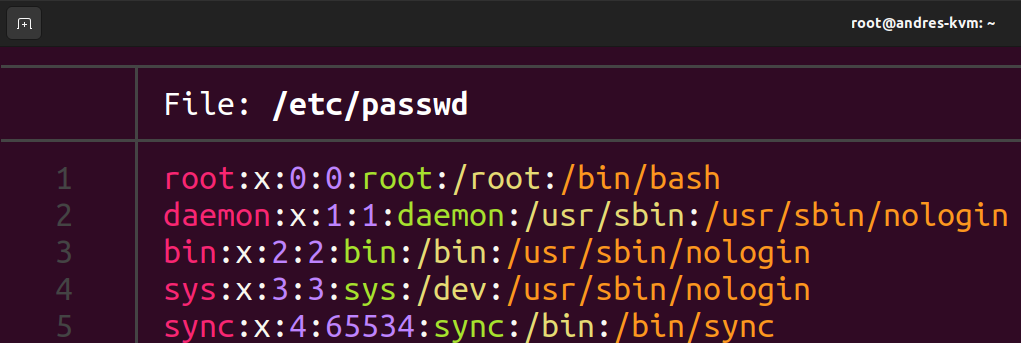
\includegraphics[width=\textwidth]{imagenes/passwdfile.png}
%    \caption{Ejemplo de entradas en el archivo.}
%\end{figure}
\section{Ejercicio 1}

\textbf{Enunciado: }``Construye y compila un programa simple, por ejemplo uno similar al “Hola, Mundo”, en dos versiones: una en C y otra en C++.''

\bigskip

Para ello voy a crear los siguientes programas:


\begin{figure}[H]
    \centering
    \begin{subfigure}{0.49\textwidth}
        \centering
        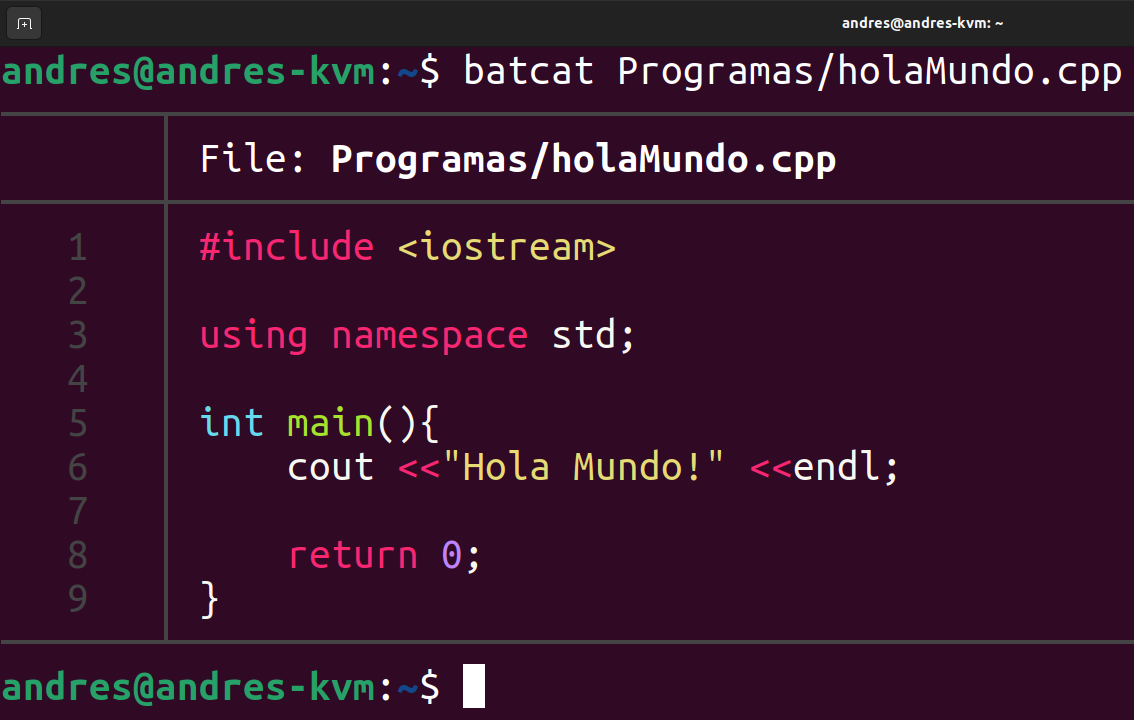
\includegraphics[width=\textwidth]{imagenes/Captura desde 2022-11-15 16-06-21.png}
        \caption{Versión C++.}
    \end{subfigure}
    \hfill
    \begin{subfigure}{0.49\textwidth}
        \centering
        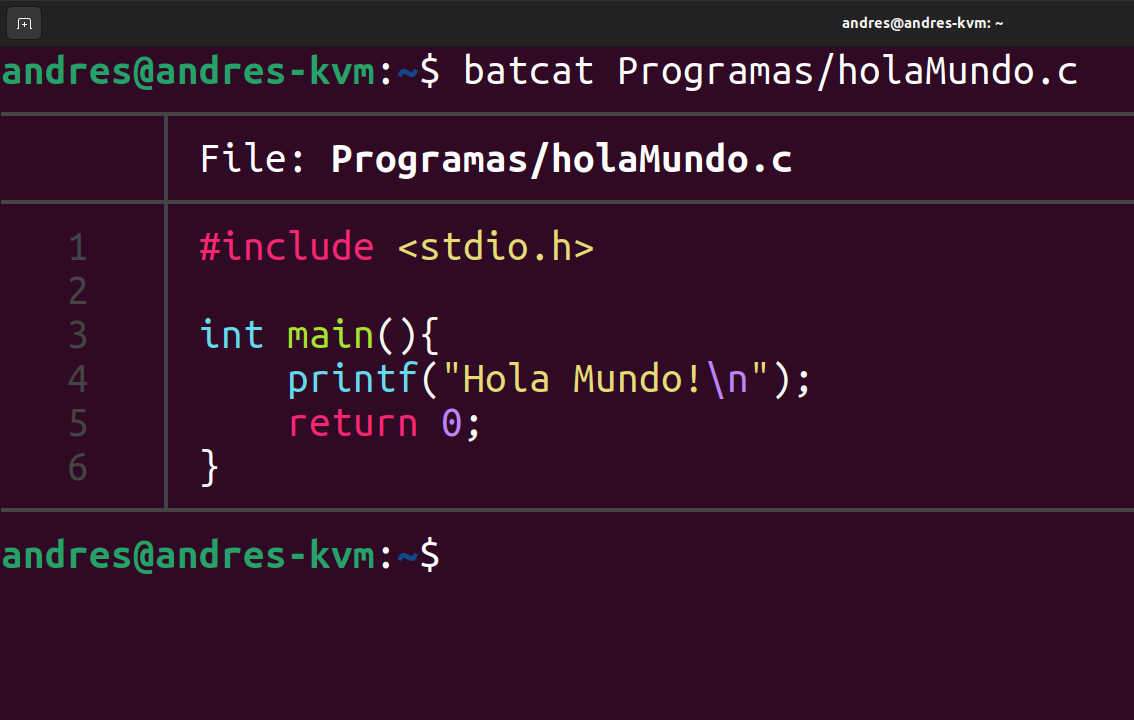
\includegraphics[width=\textwidth]{imagenes/Captura desde 2022-11-15 16-06-14.png}
        \caption{Versión C.}
    \end{subfigure}

    \caption{Distintas versiones del programa.}
\end{figure}



Y voy a usar las siguientes órdenes para compilarlos:

\bigskip

\verb|g++ -o salidaCPP holaMundo.cpp|

\verb|gcc -o salidaC holaMundo.c|

\bigskip


\subsection{Apartado A}

\textbf{Enunciado: }``Consulta los manuales, o en Internet que contienen las secciones \texttt{.interp}, \texttt{.got}, \texttt{got.ptl}.''

\bigskip

A continuación explicaré que contiene cada sección, para obtener información se puede usar la orden \verb|man 5 elf|:

\begin{itemize}
    \item \textbf{.interp}: Esta sección almacena la ruta del intérprete del programa. Si el archivo tiene un segmento que incluye esta sección, los atributos de la sección tendrán el bit \texttt{SHF\_ALLOC}. La sección es de tipo \texttt{SHT\_PROGBITS}.
    
    \item \textbf{.got}: Esta sección almacena la tabla de desplazamientos global (Global Offset Table). Es de tipo \texttt{SH\_PROGBITS} y sus atributos son específicos del procesador. 
    
    \item \textbf{.got.plt}: Esta sección almacena la tabla de vinculación de procedimientos (Procedure Linkage Table). Es de tipo \texttt{SH\_PROGBITS} y sus atributos son específicos del procesador. Sirve para obtener las direcciones a funciones para posteriormente poder ser llamadas.
\end{itemize}

\newpage
\subsection{Apartado B}

\textbf{Enunciado: }``Compara los ELFs de las dos versiones listando las secciones ¿hay alguna diferencia relevante respecto a las secciones de un programa compilado con gcc? ¿qué contienen las secciones \texttt{.ctors} y \texttt{.dtors}?''

\bigskip

Ejecutando la orden \verb|readelf -S ejecutable| podemos obtener las secciones que componen el programa.

\begin{figure}[H]
    \centering
    \begin{subfigure}{0.49\textwidth}
        \centering
        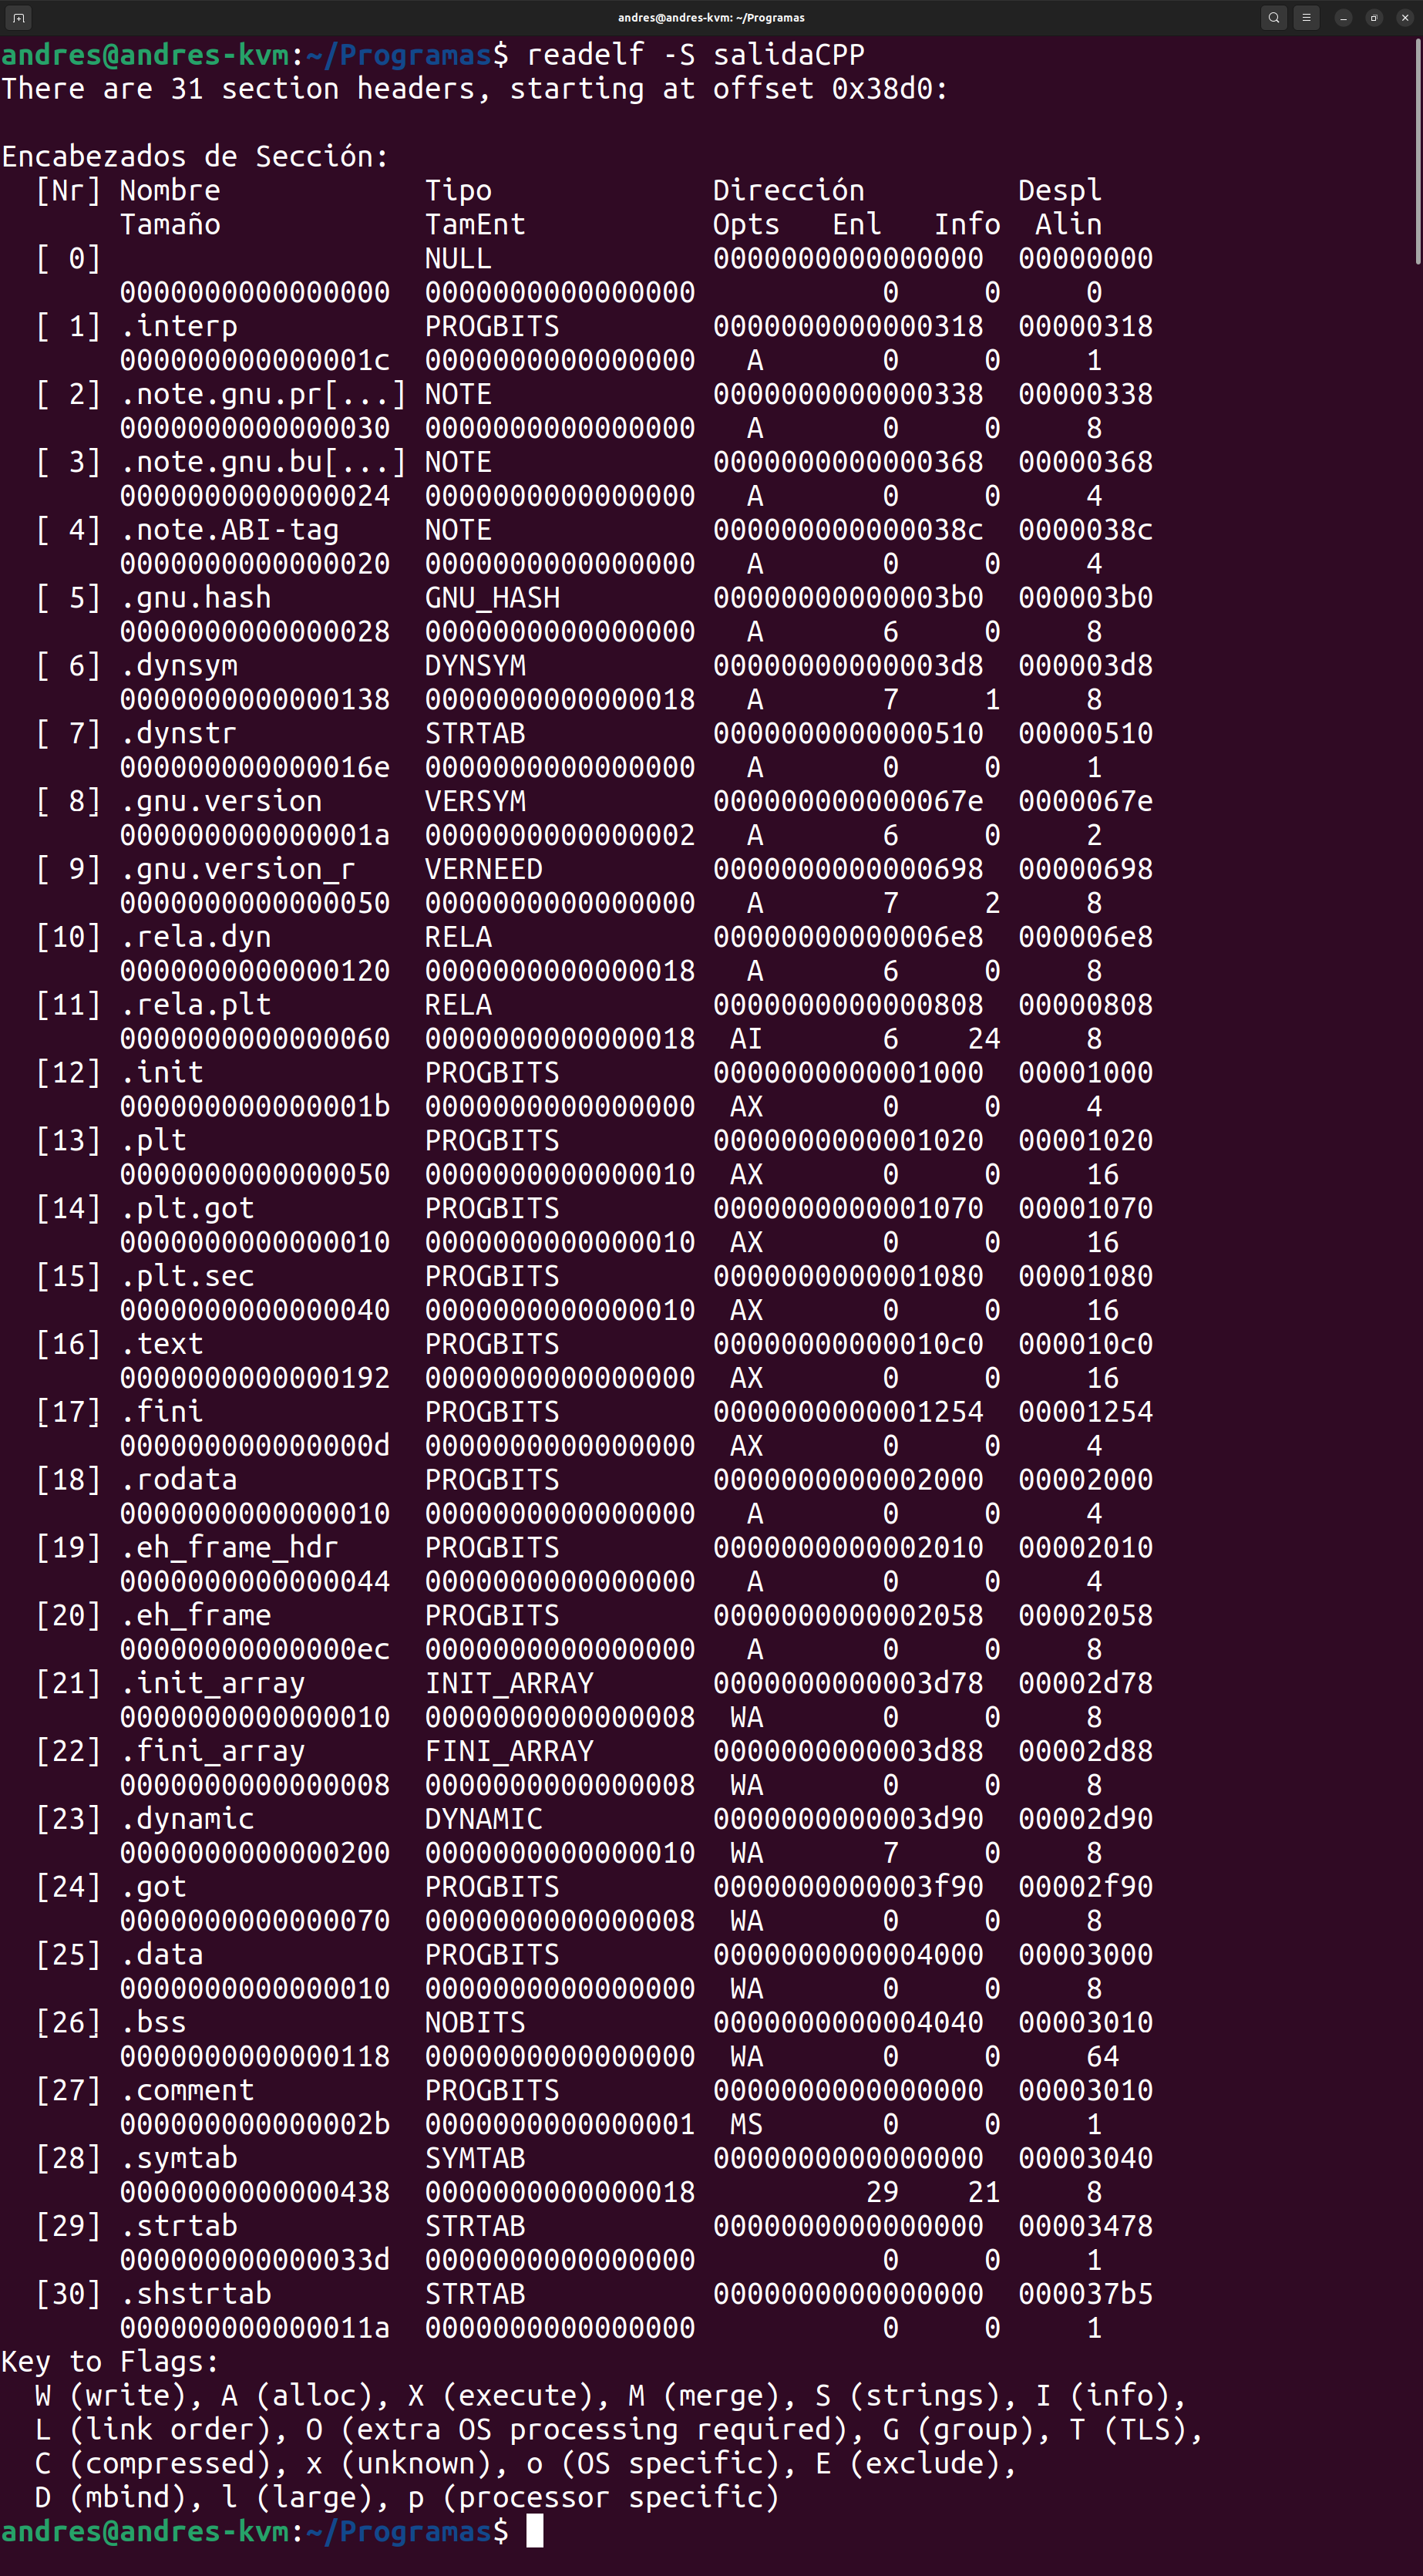
\includegraphics[width=\textwidth]{imagenes/CPP/merged.png}
        \caption{Versión C++.}
    \end{subfigure}
    \hfill
    \begin{subfigure}{0.49\textwidth}
        \centering
        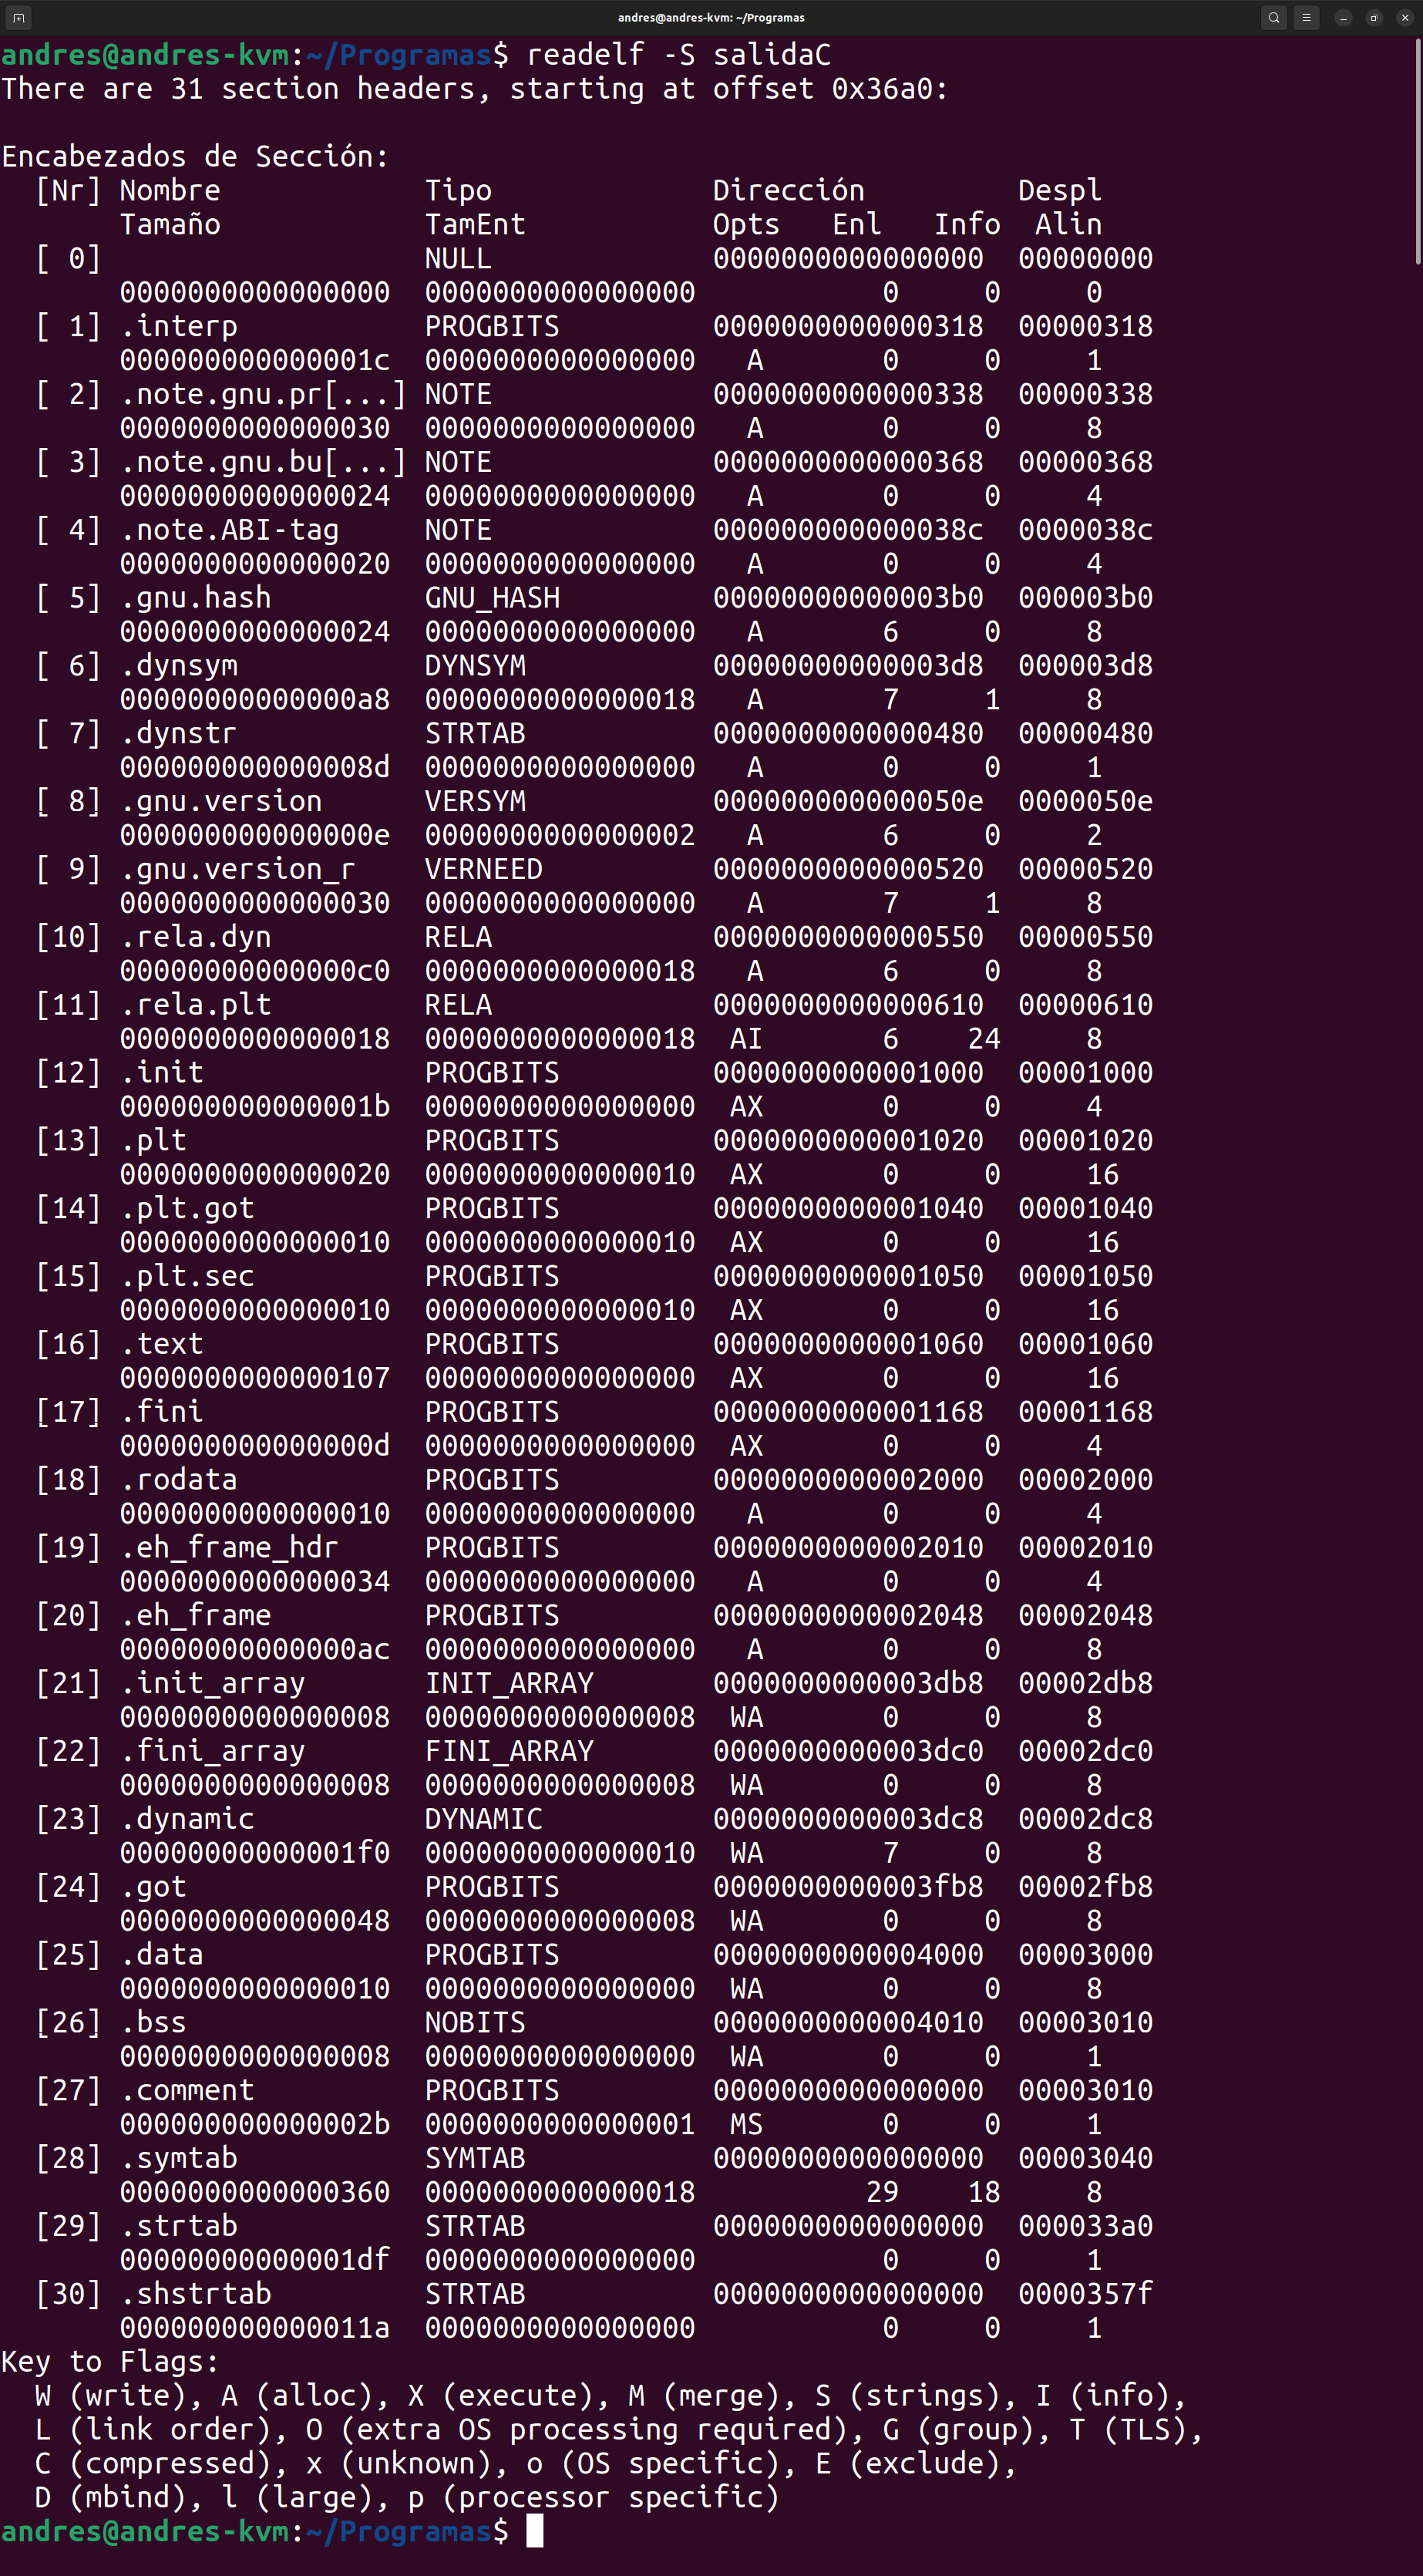
\includegraphics[width=\textwidth]{imagenes/C/merged.png}
        \caption{Versión C.}
    \end{subfigure}

    \caption{Secciones de los programas.}
\end{figure}

\newpage

Ahora, para mostrar por terminal la diferencia de los archivos a color se puede usar la orden \verb|icdiff archivo1 archivo2|.

%foto de icdiff (quizas haya que cortarlas)
\begin{figure}[H]
    \centering
    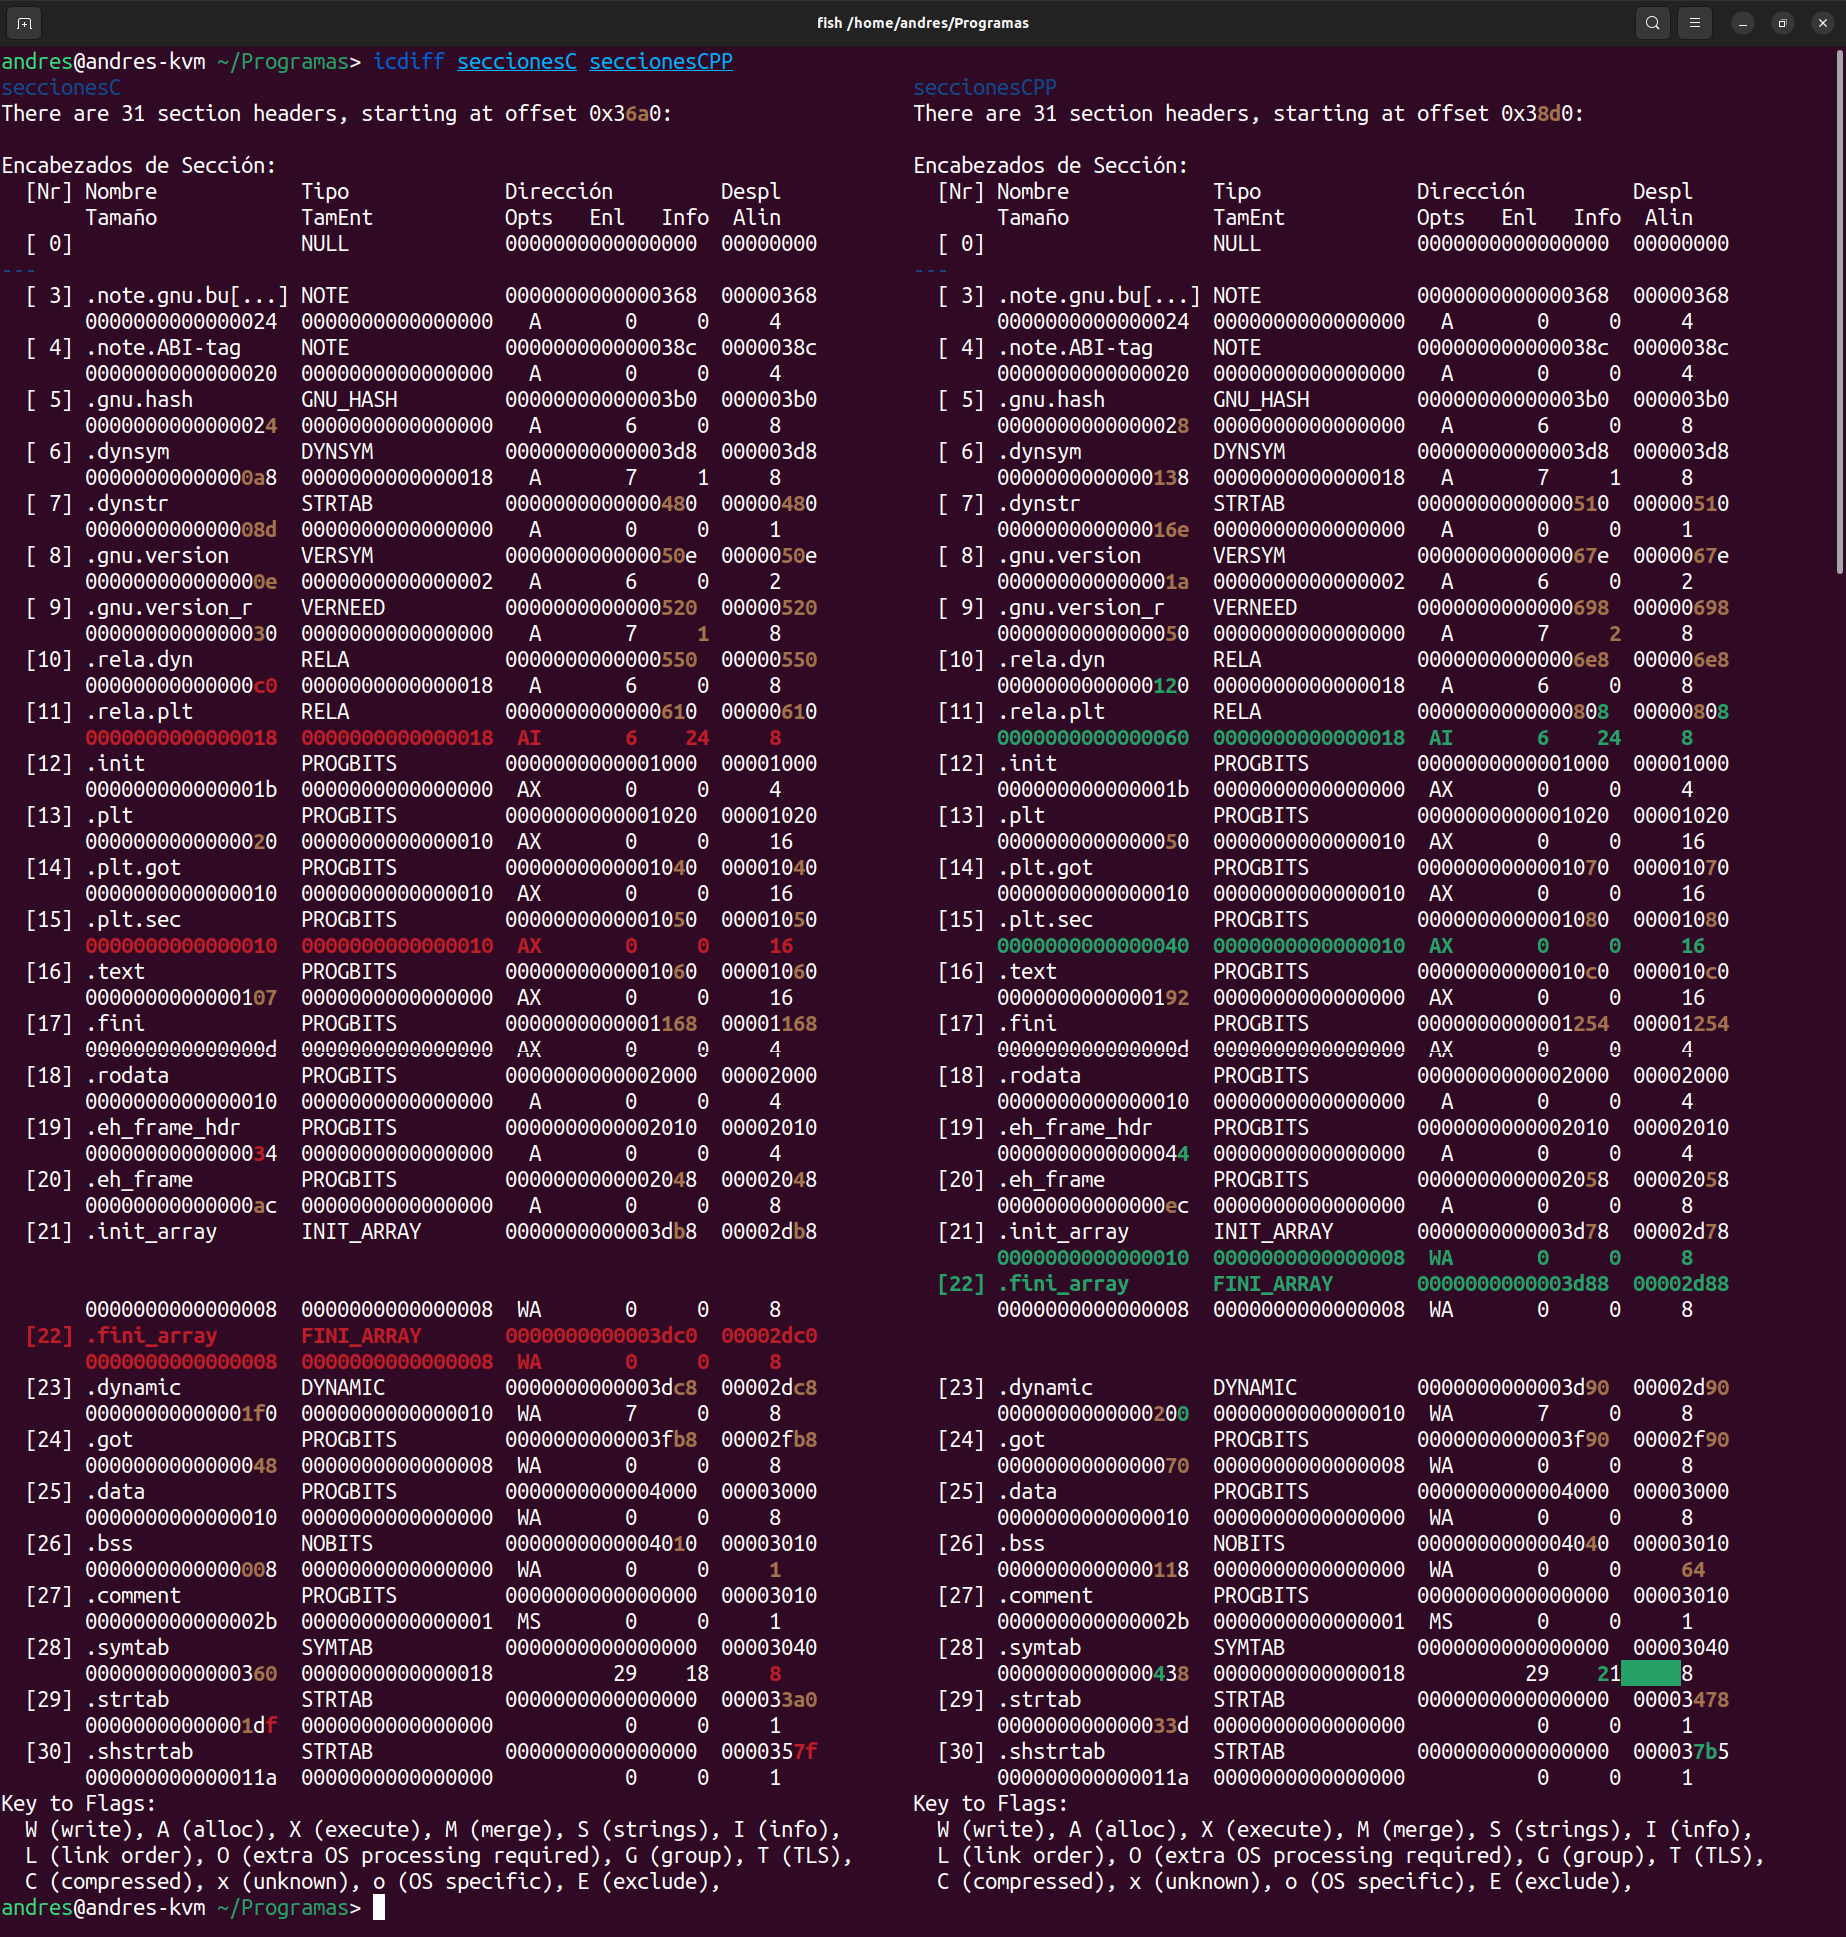
\includegraphics[width=0.95\textwidth]{imagenes/icdiff/mergedicdiff.png}
    \caption{Diferencias entre ambas versiones compiladas.}
\end{figure}

Como se puede ver, en la primera línea, el offset es distinto, siendo más alto en el programa escrito en C++. Además, se puede ver que algunas secciones del programa escrito en C++ son ligeramente más grandes que la versión en C. Estas secciones son: \textbf{.gun.hash, .dynsym, .dynstr, .gun.version, .rela.dyn, .rela.plt, .plt, .plt.sec, .text, .eh\_frame\_hdr, .eh\_frame, .init\_array, .fini\_array, .dynamic, .got, .bss, .symtab, y .strtab.}

\bigskip

Por último, se puede ver que el desplazamiento (offset) y las direcciones de memoria de estas secciones varía entre una versión y otra.


\bigskip

Las secciones .ctors y .dtors contienen lo siguiente:

\begin{itemize}
    \item \textbf{.ctors}: Esta sección almacena punteros inicializados a las funciones del constructor de C++ (constructores de las clases).
    \item \textbf{.dtors}: Esta sección almacena punteros inicializados a las funciones del destructor de C++ (destructores de las clases).
\end{itemize}

\newpage

\subsection{Apartado C}

\textbf{Enunciado: }``Con la opción \texttt{readelf -r} podemos ver las secciones de reubicación. Indicar que contienen estas secciones.''

\bigskip

Mediante la orden \verb|readelf -r programa| podemos ver las distintas secciones que contiene. Estas son:

\begin{itemize}
    \item \textbf{.rela.dyn}: Contiene las entradas de reubicación para símbolos dinámicos; es decir, estas variables deben ser reubicadas en tiempo de ejecución.
    \item \textbf{.rela.plt}: Contiene las entradas de reubicación para símbolos de funciones. Al igual que el anterior, deben ser reubicadas en tiempo de ejecución.
\end{itemize}

Además, la versión de C++ tiene más entradas que la versión de C, como pasó en el apartado anterior.

\bigskip

\section{Ejercicio 2}

\textbf{Enunciado: }``Mira en el manual en línea o en Internet las opciones de la orden objdump, e indica:''

\subsection{Apartado A}

\textbf{Enunciado: }``qué opciones nos permiten ver la información que nos suministra \texttt{readelf}.''

\bigskip

El comando \verb|objdump| tiene algunos switches similares a los de \verb|readelf|. A continuación voy a indicar algunos que se han usado en el ejercicio anterior:

\begin{itemize}
    \item \verb|readelf -r <archivo>| $\rightarrow$ \verb|objdump -Rr <archivo>|
    
    
    Muestra las entradas de reubicación del archivo ELF.

    %foto readelf y objdump side by side
    \begin{figure}[H]
        \centering
        \begin{subfigure}{0.49\textwidth}
            \centering
            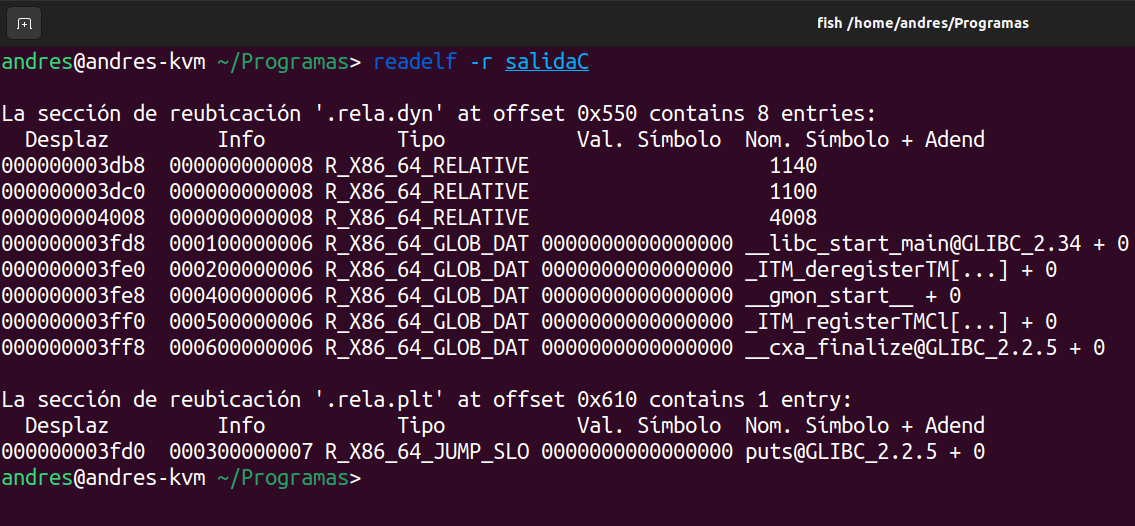
\includegraphics[width=\textwidth]{imagenes/Captura desde 2022-11-17 17-42-30.png}
            \caption{Versión \texttt{readelf}.}
        \end{subfigure}
        \hfill
        \begin{subfigure}{0.49\textwidth}
            \centering
            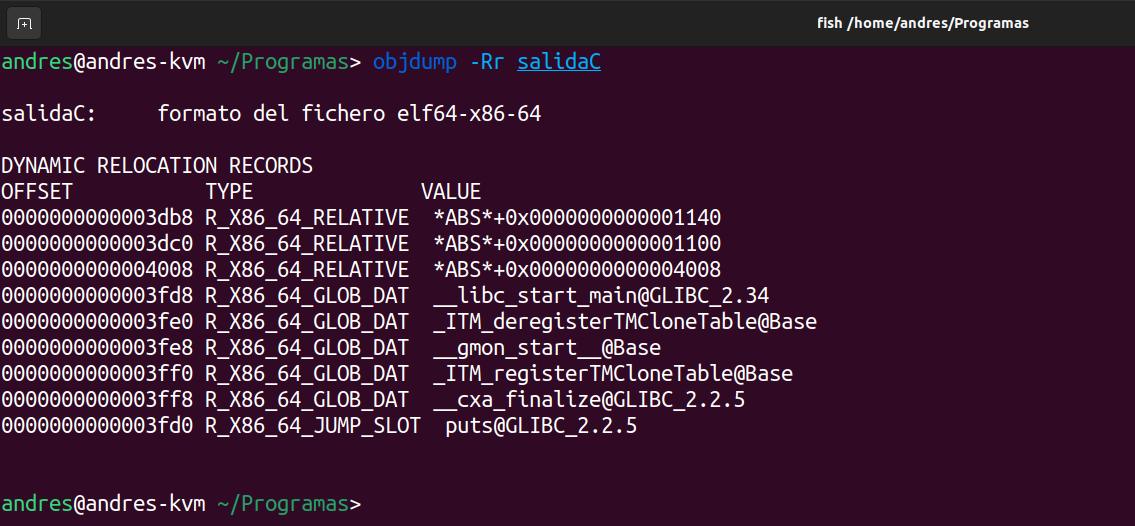
\includegraphics[width=\textwidth]{imagenes/Captura desde 2022-11-17 17-42-36.png}
            \caption{Versión \texttt{objdump}.}
        \end{subfigure}
        \caption{Salida de ambas versiones.}
    \end{figure}

    \newpage

    \item \verb|readelf -h <archivo>| $\rightarrow$ \verb|objdump -f <archivo>|
    
    Muestra las cabeceras del propio archivo ELF.

    %foto side by side
    \begin{figure}[H]
        \centering
        \begin{subfigure}{0.49\textwidth}
            \centering
            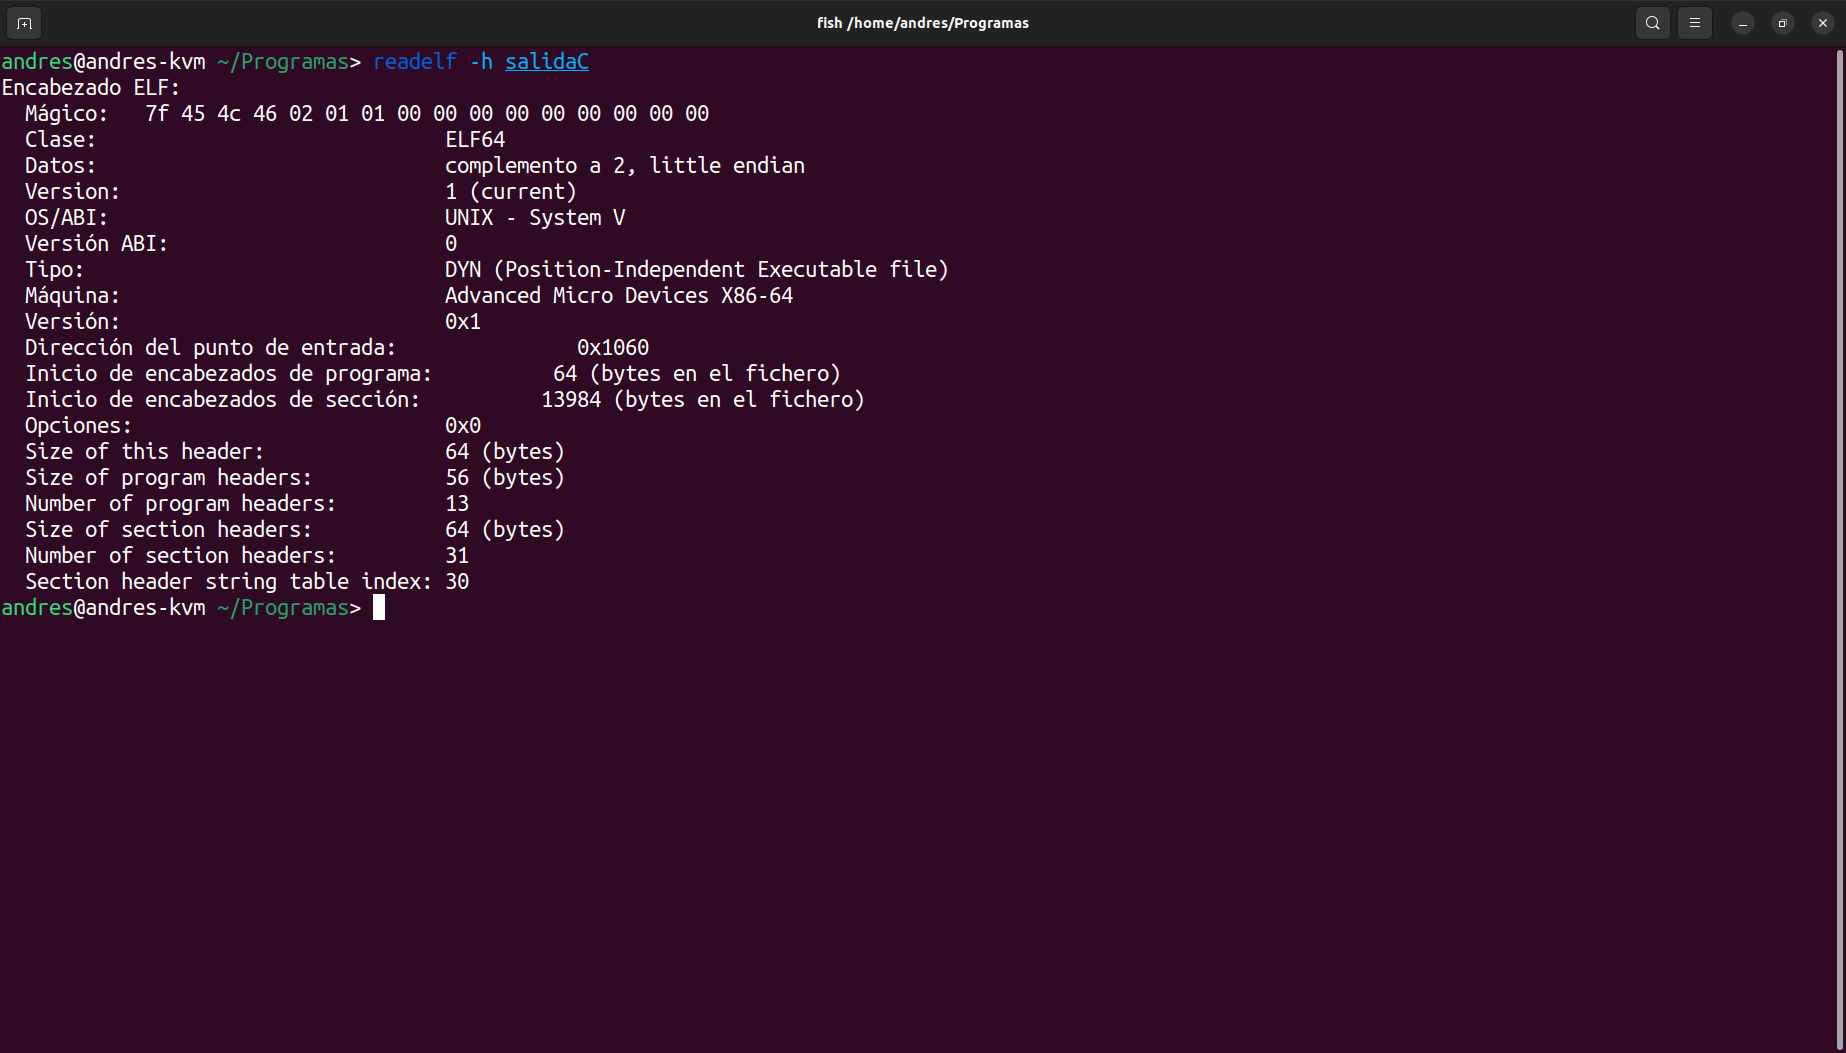
\includegraphics[width=\textwidth]{imagenes/Captura desde 2022-11-17 17-44-04.png}
            \caption{Versión \texttt{readelf}.}
        \end{subfigure}
        \hfill
        \begin{subfigure}{0.49\textwidth}
            \centering
            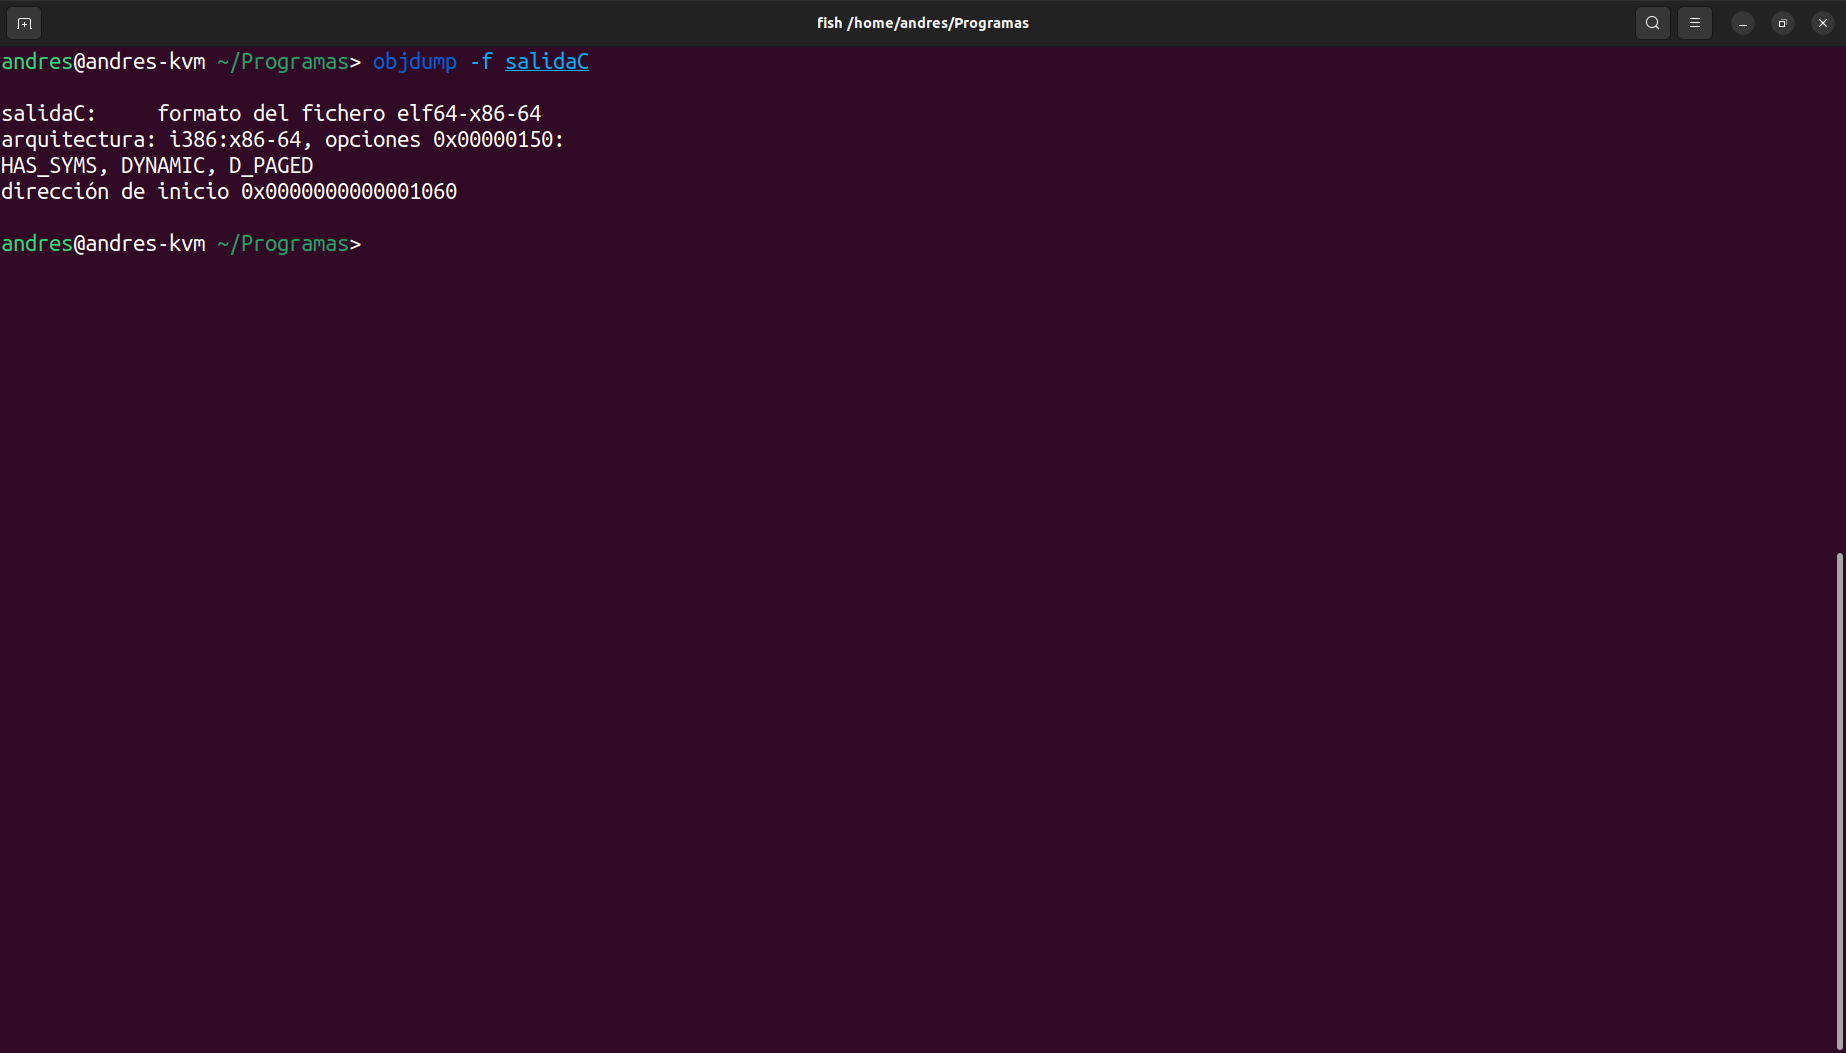
\includegraphics[width=\textwidth]{imagenes/Captura desde 2022-11-17 17-44-19.png}
            \caption{Versión \texttt{objdump}.}
        \end{subfigure}
        \caption{Salida de ambas versiones.}
    \end{figure}

    \item \verb|readelf -S <archivo>| $\rightarrow$ \verb|objdump -h <archivo>|
    
    Muestra la información de las cabeceras de sección (section headers).

    %foto side by side
    \begin{figure}[H]
        \centering
        \begin{subfigure}{0.45\textwidth}
            \centering
            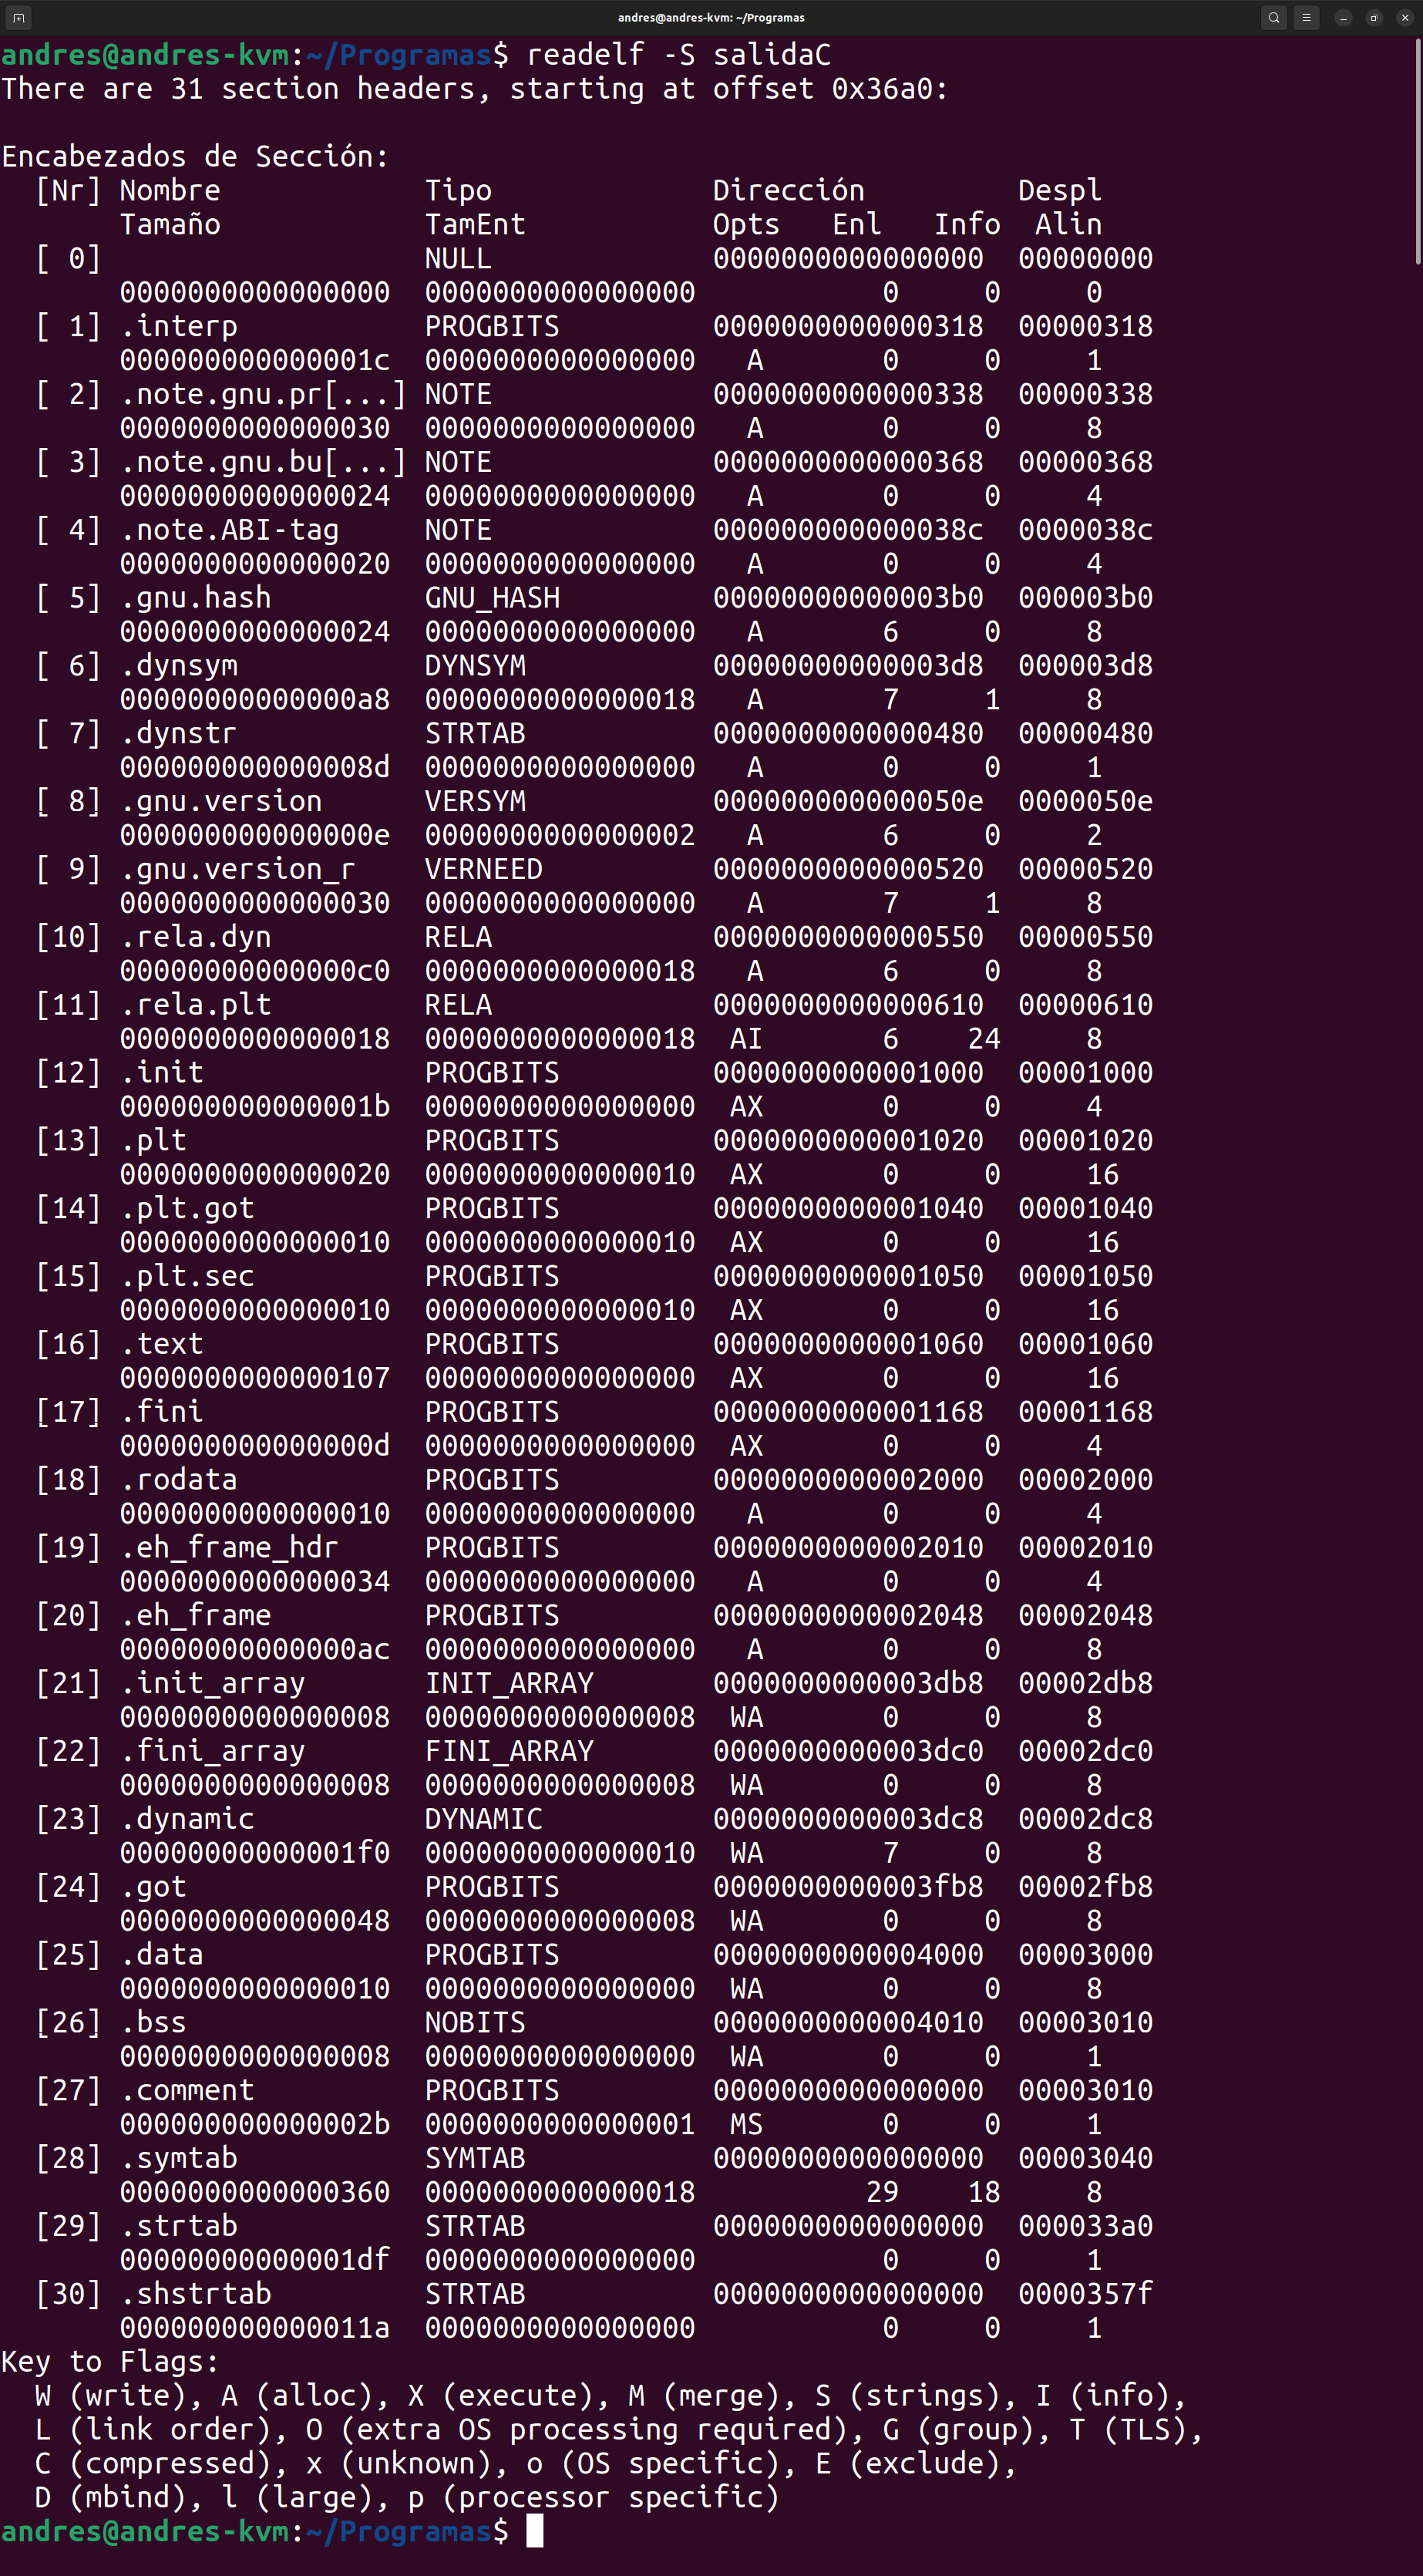
\includegraphics[width=\textwidth]{imagenes/C/merged.png}
            \caption{Versión \texttt{readelf}.}
        \end{subfigure}
        \hfill
        \begin{subfigure}{0.45\textwidth}
            \centering
            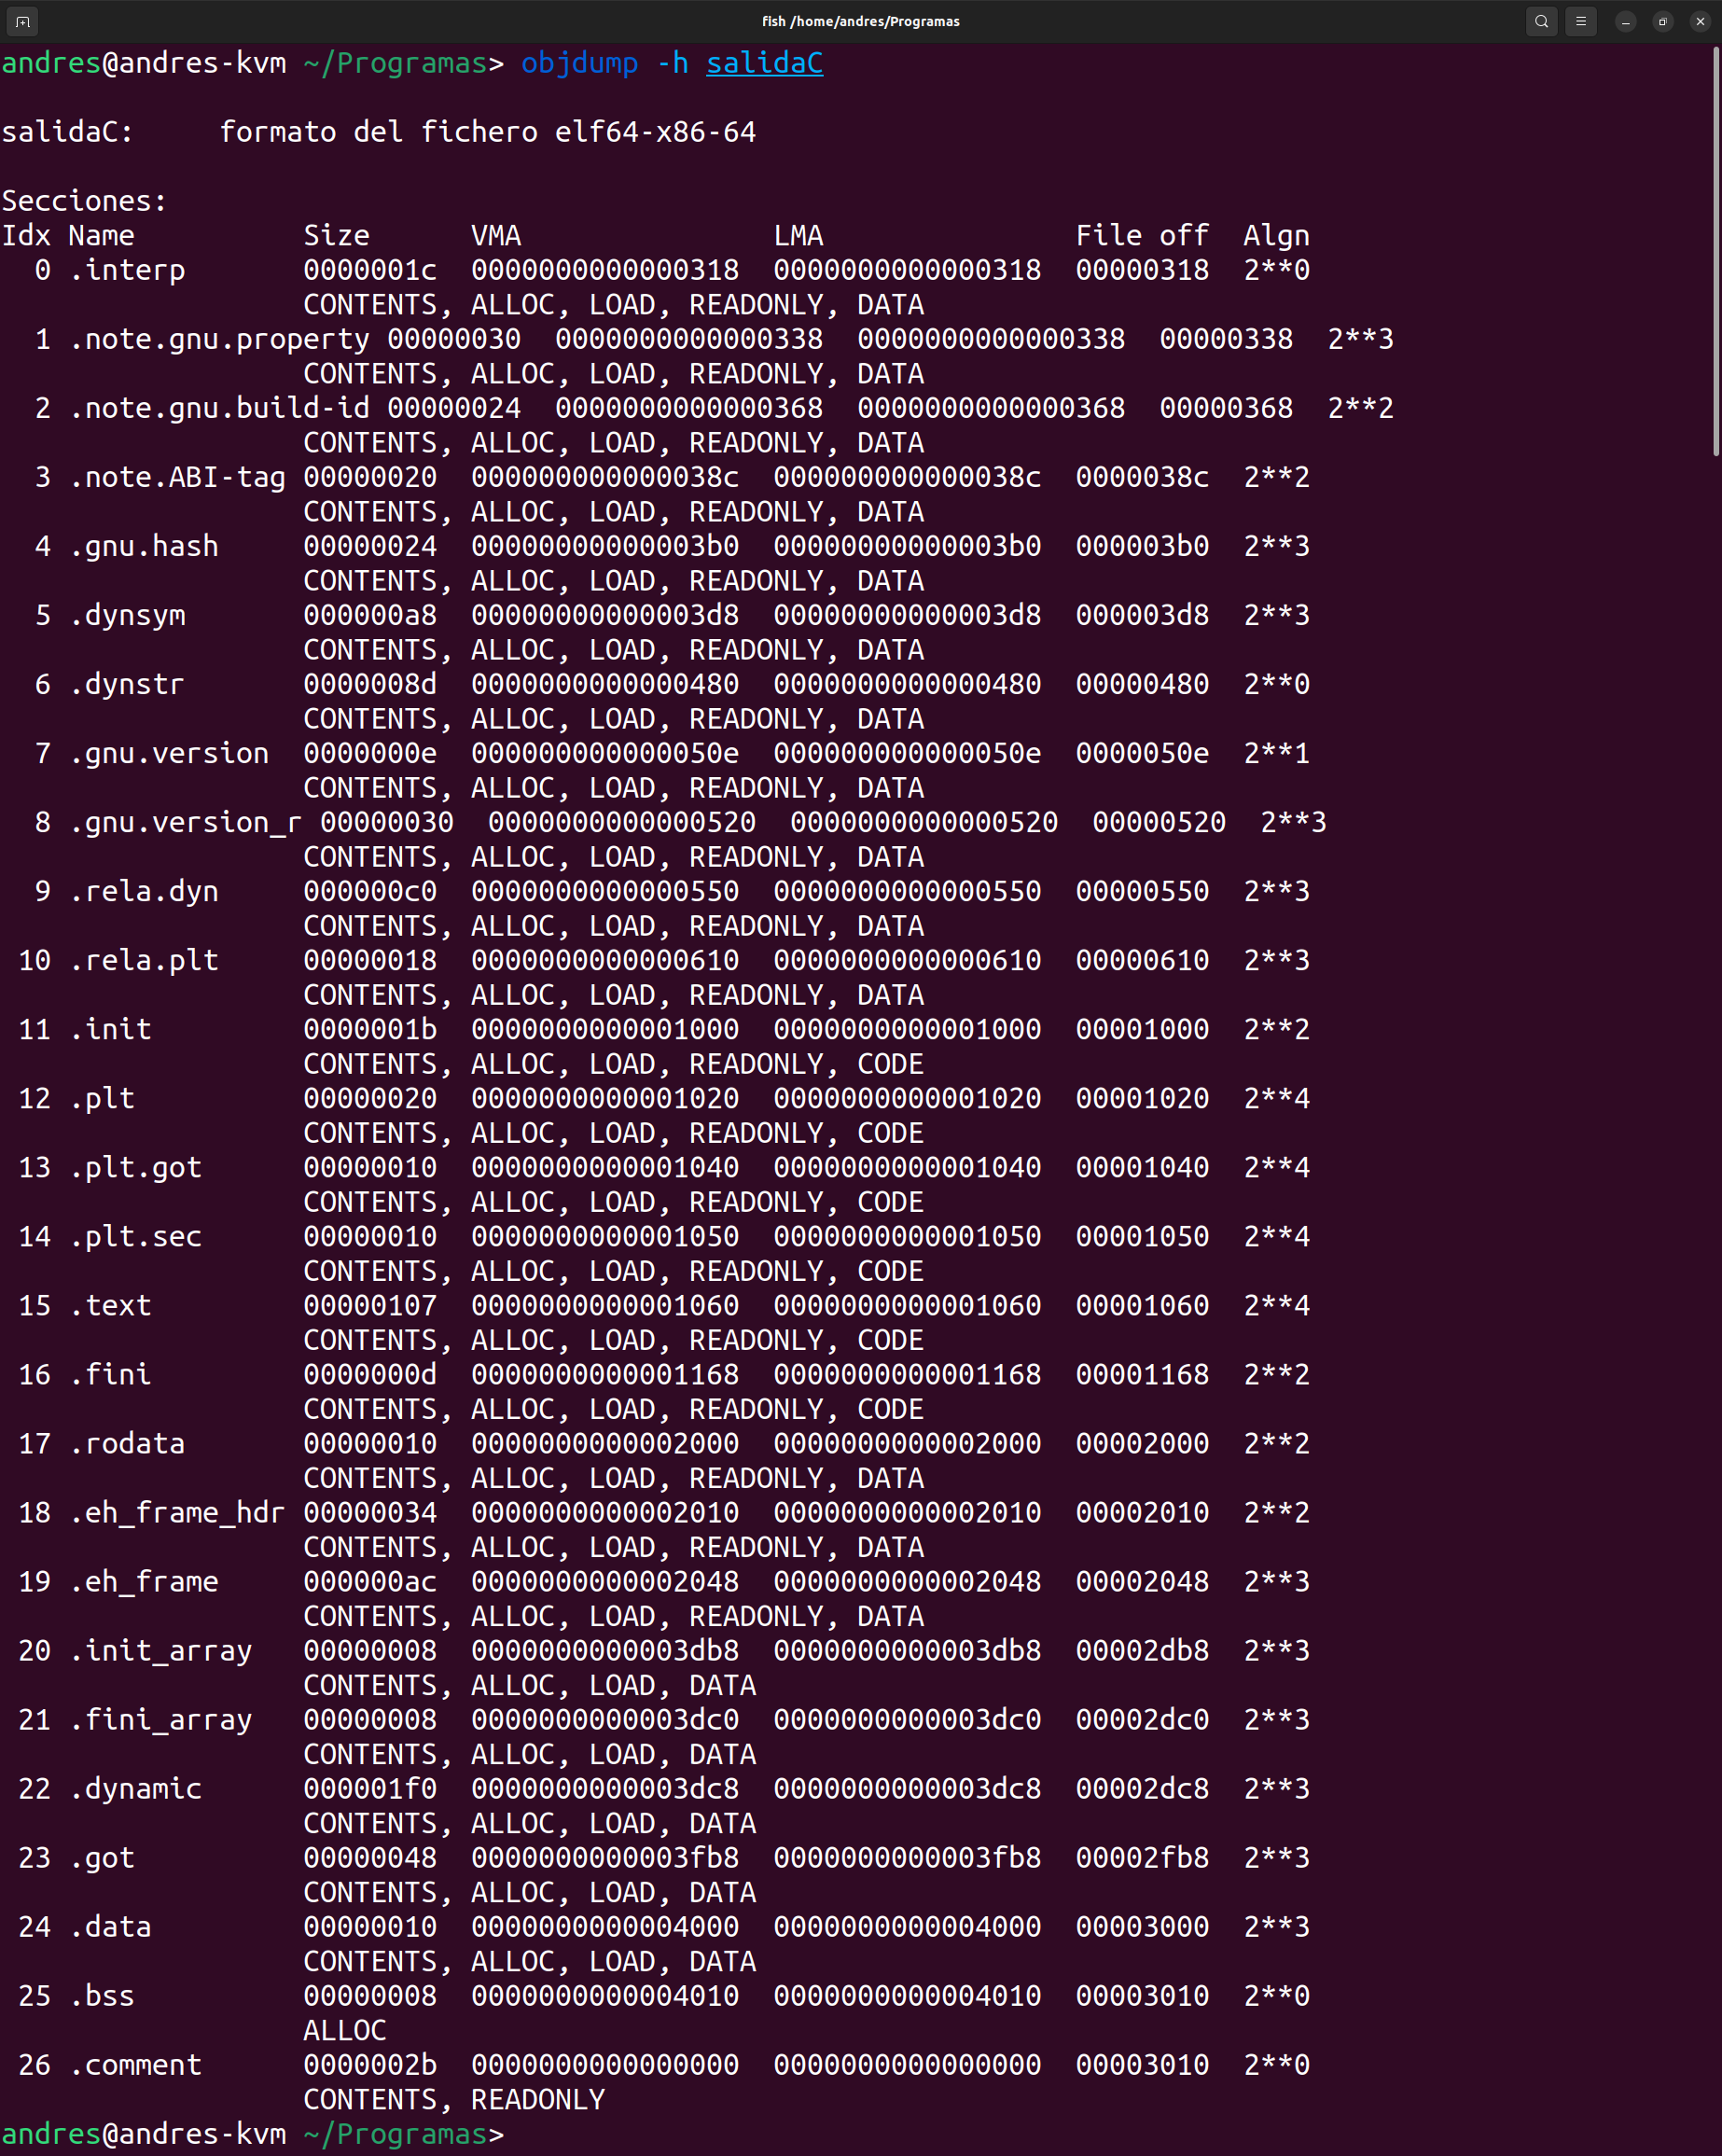
\includegraphics[width=\textwidth]{imagenes/merged.png}
            \caption{Versión \texttt{objdump}.}
        \end{subfigure}
        \caption{Salida de ambas versiones.}
    \end{figure}

    \newpage

    \item \verb|readelf -l <archivo>| $\rightarrow$ \verb|objdump -p <archivo>|
    
    Muestra las cabeceras del programa.

    %foto side by side
    \begin{figure}[H]
        \centering
        \begin{subfigure}{0.49\textwidth}
            \centering
            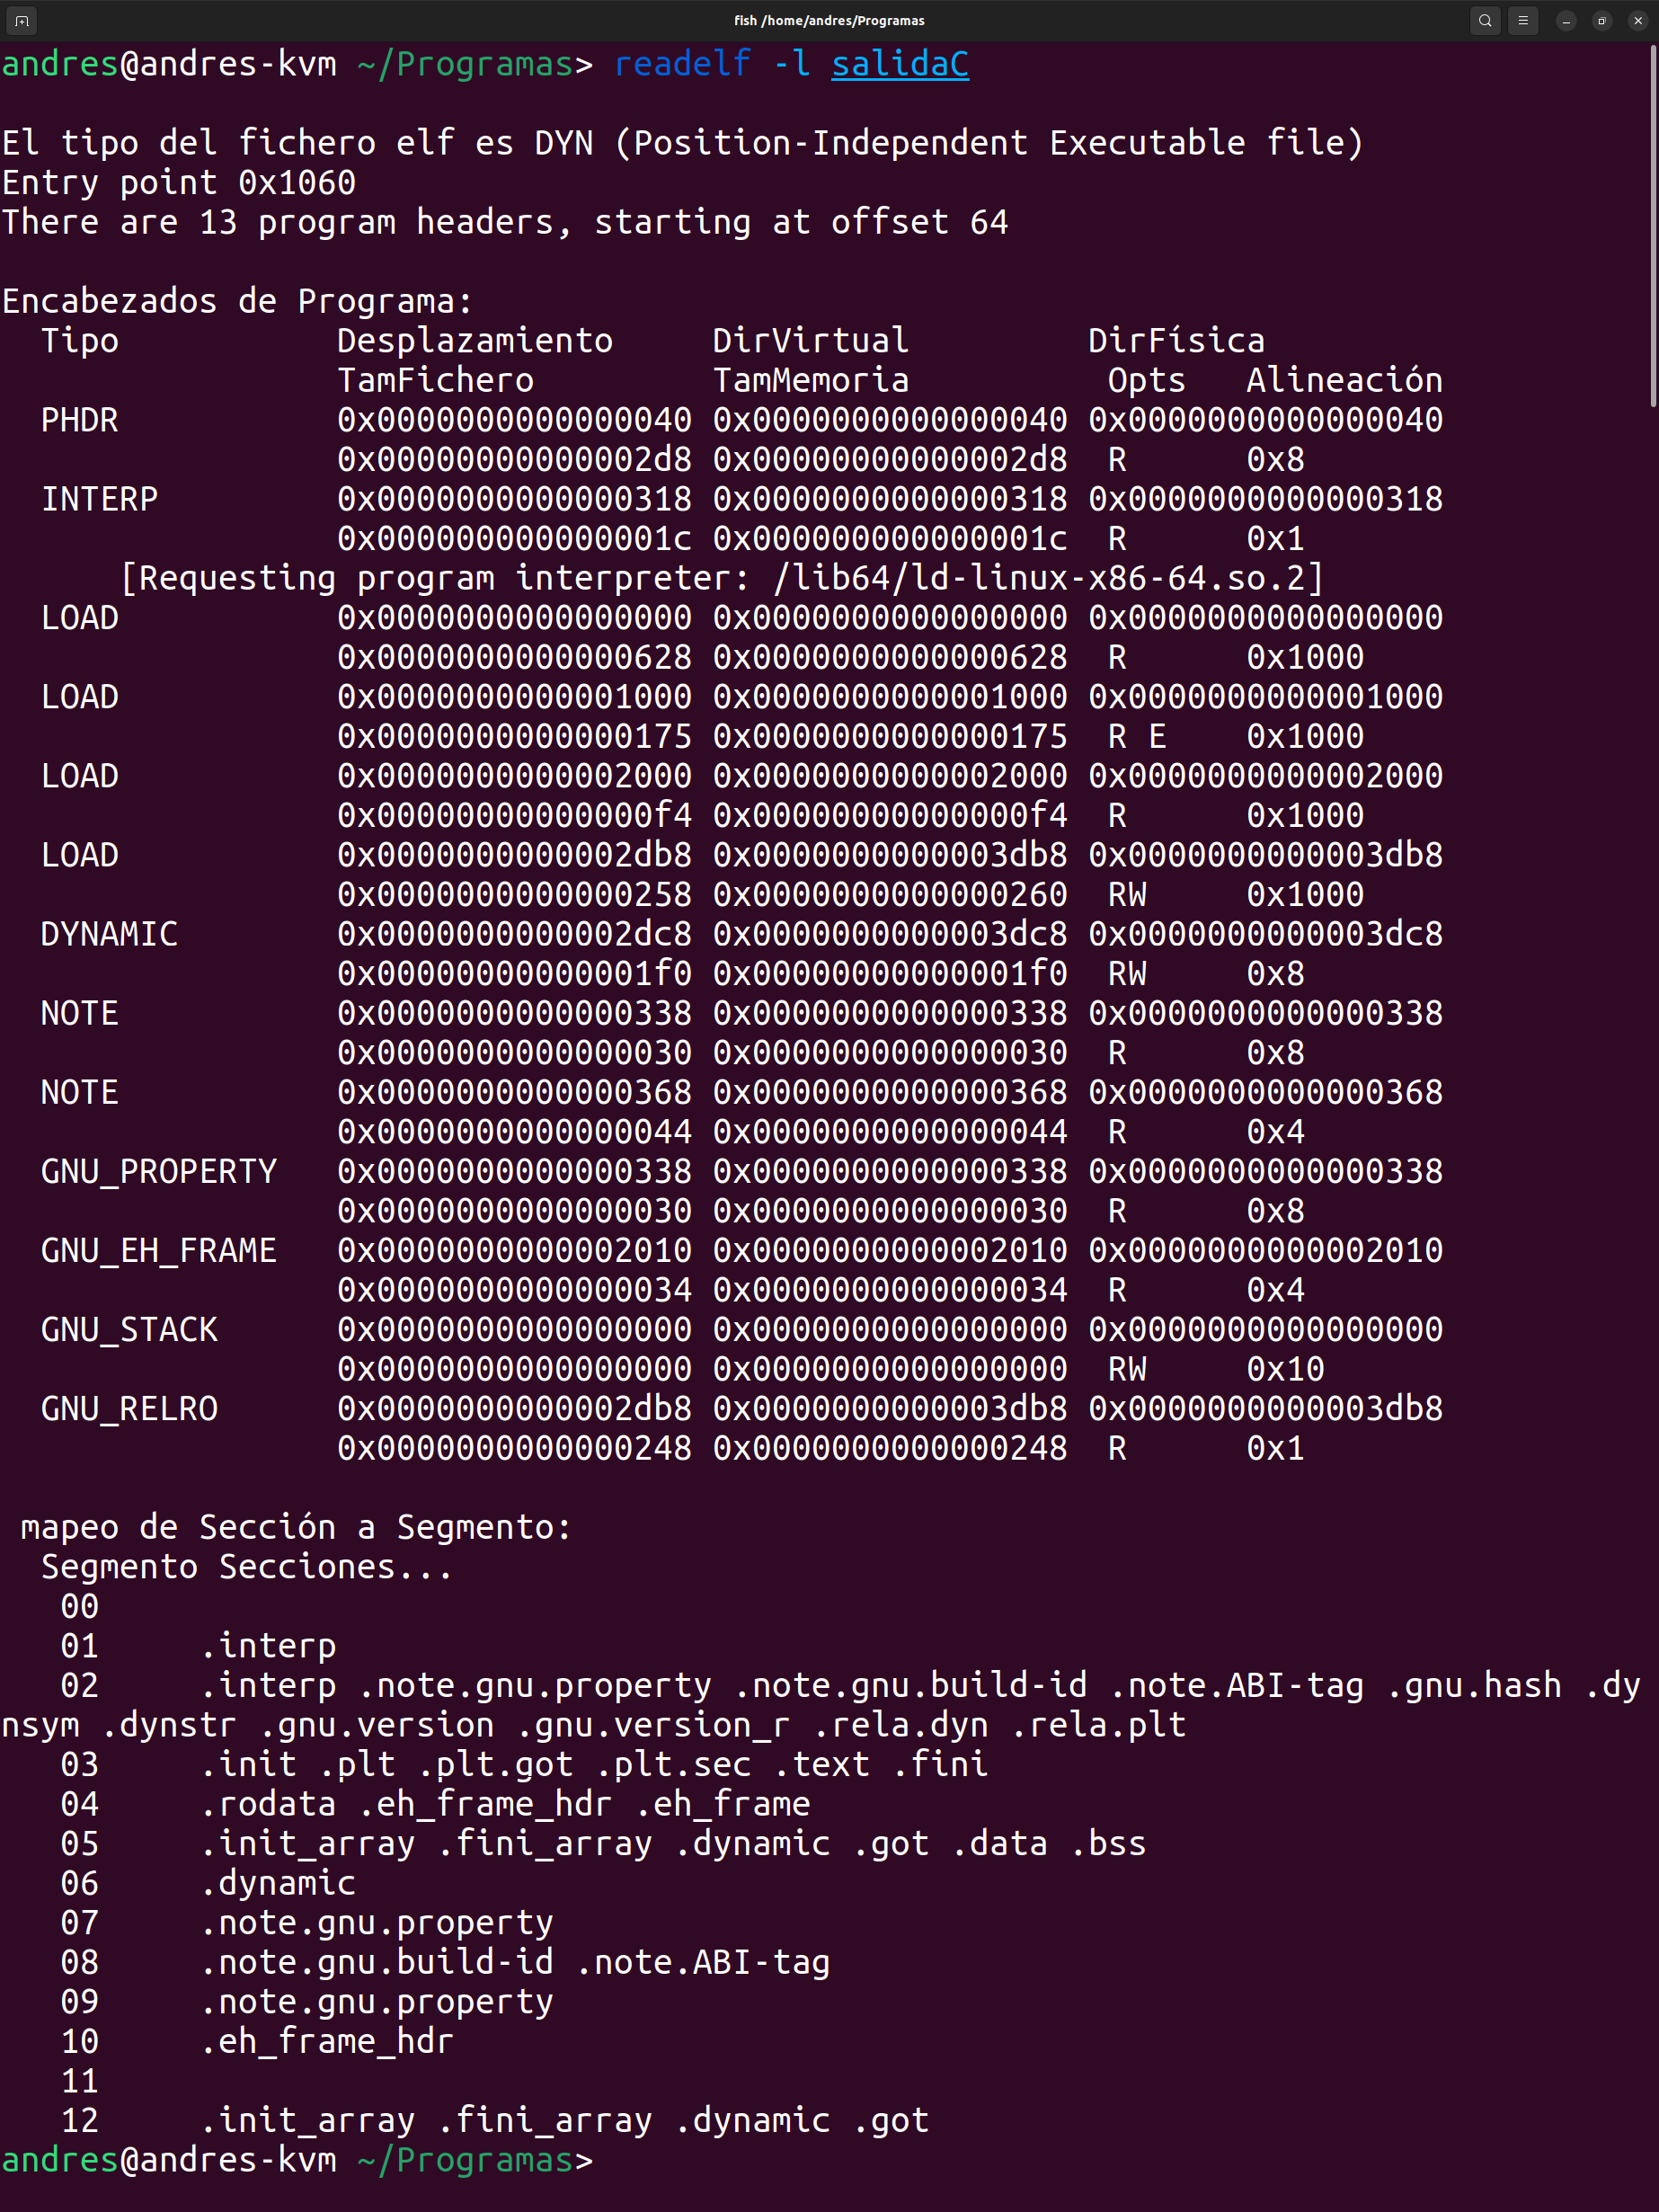
\includegraphics[width=\textwidth]{imagenes/mergedelfl.png}
            \caption{Versión \texttt{readelf}.}
        \end{subfigure}
        \hfill
        \begin{subfigure}{0.49\textwidth}
            \centering
            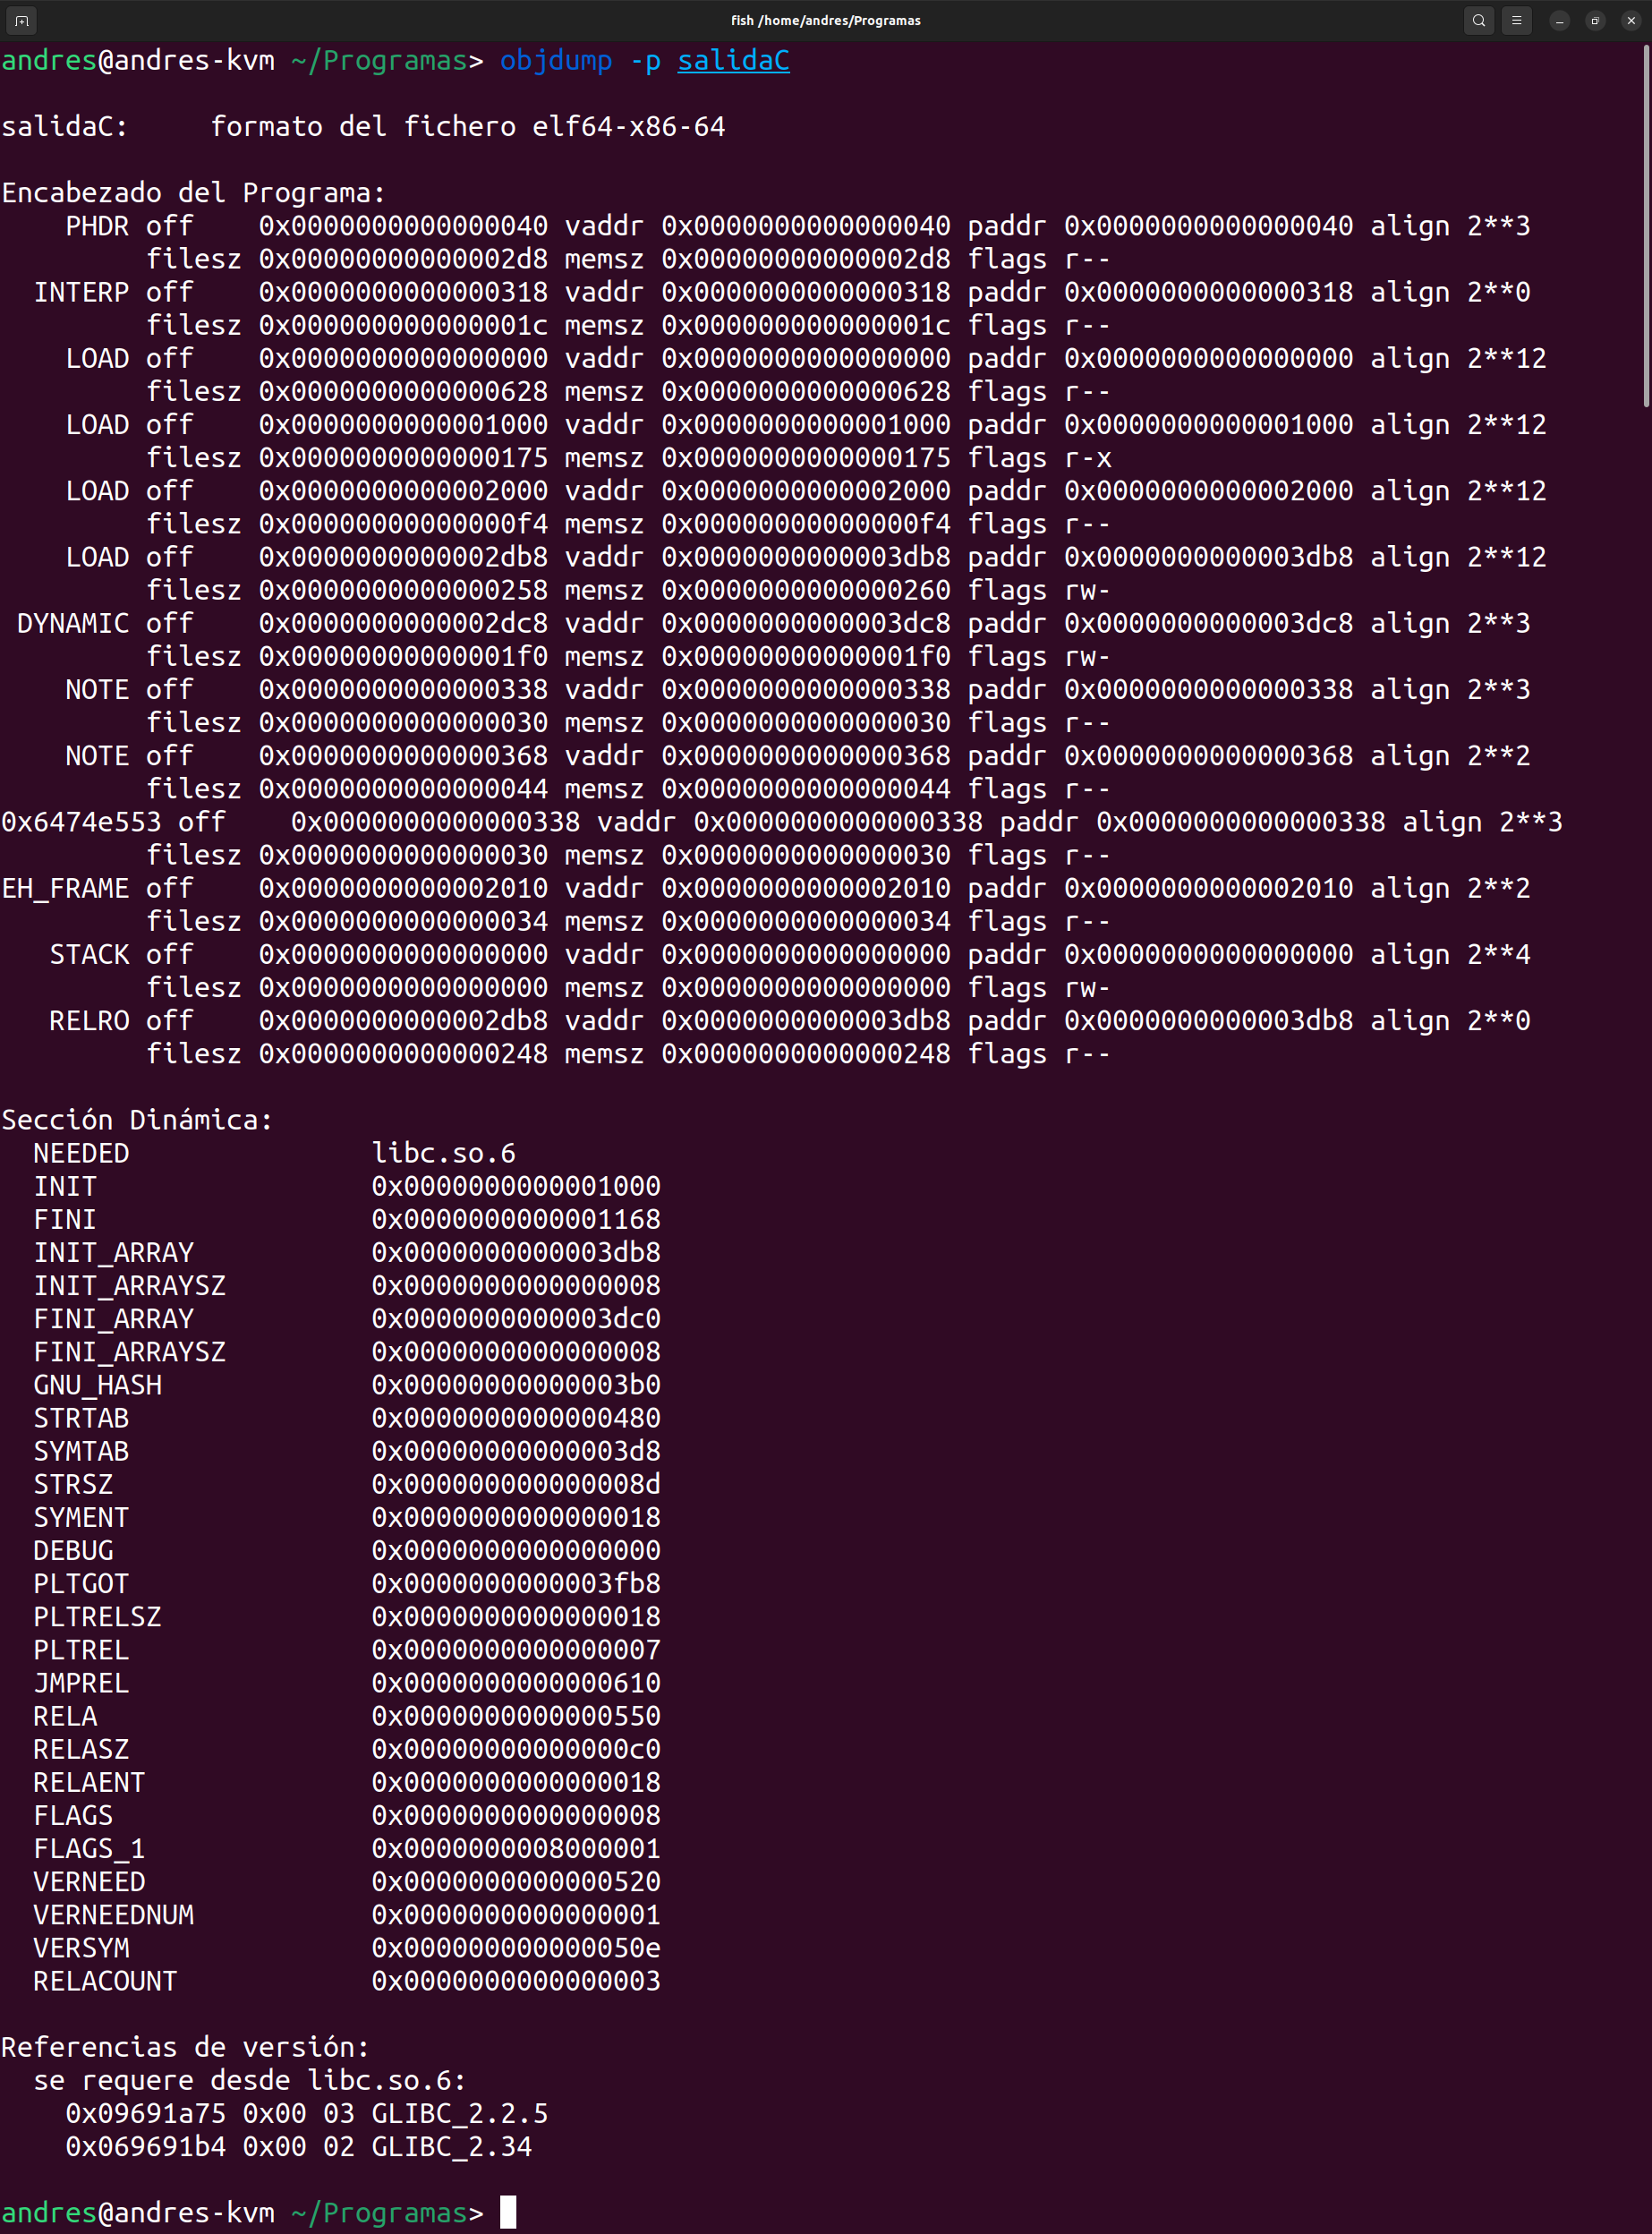
\includegraphics[width=\textwidth]{imagenes/mergedobjdumpp}
            \caption{Versión \texttt{objdump}.}
        \end{subfigure}
        \caption{Salida de ambas versiones.}
    \end{figure}    

\end{itemize}

% TABLE: READELF VS OBJDUMP
% -r / -Rr
% -h / -f
% -S / -h
% -l / -p

\subsection{Apartado B}

\textbf{Enunciado: }``qué otras opciones nos permite realizar \texttt{objdump} desde el punto de la ingeniería inversa.''

\bigskip

Esta herramienta sirve de mucha utilidad desde el punto de ingeniería inversa, ya que permite el desensamblado de un ejecutable en las instrucciones máquina que lo compone.

%foto de eso
\begin{figure}[H]
    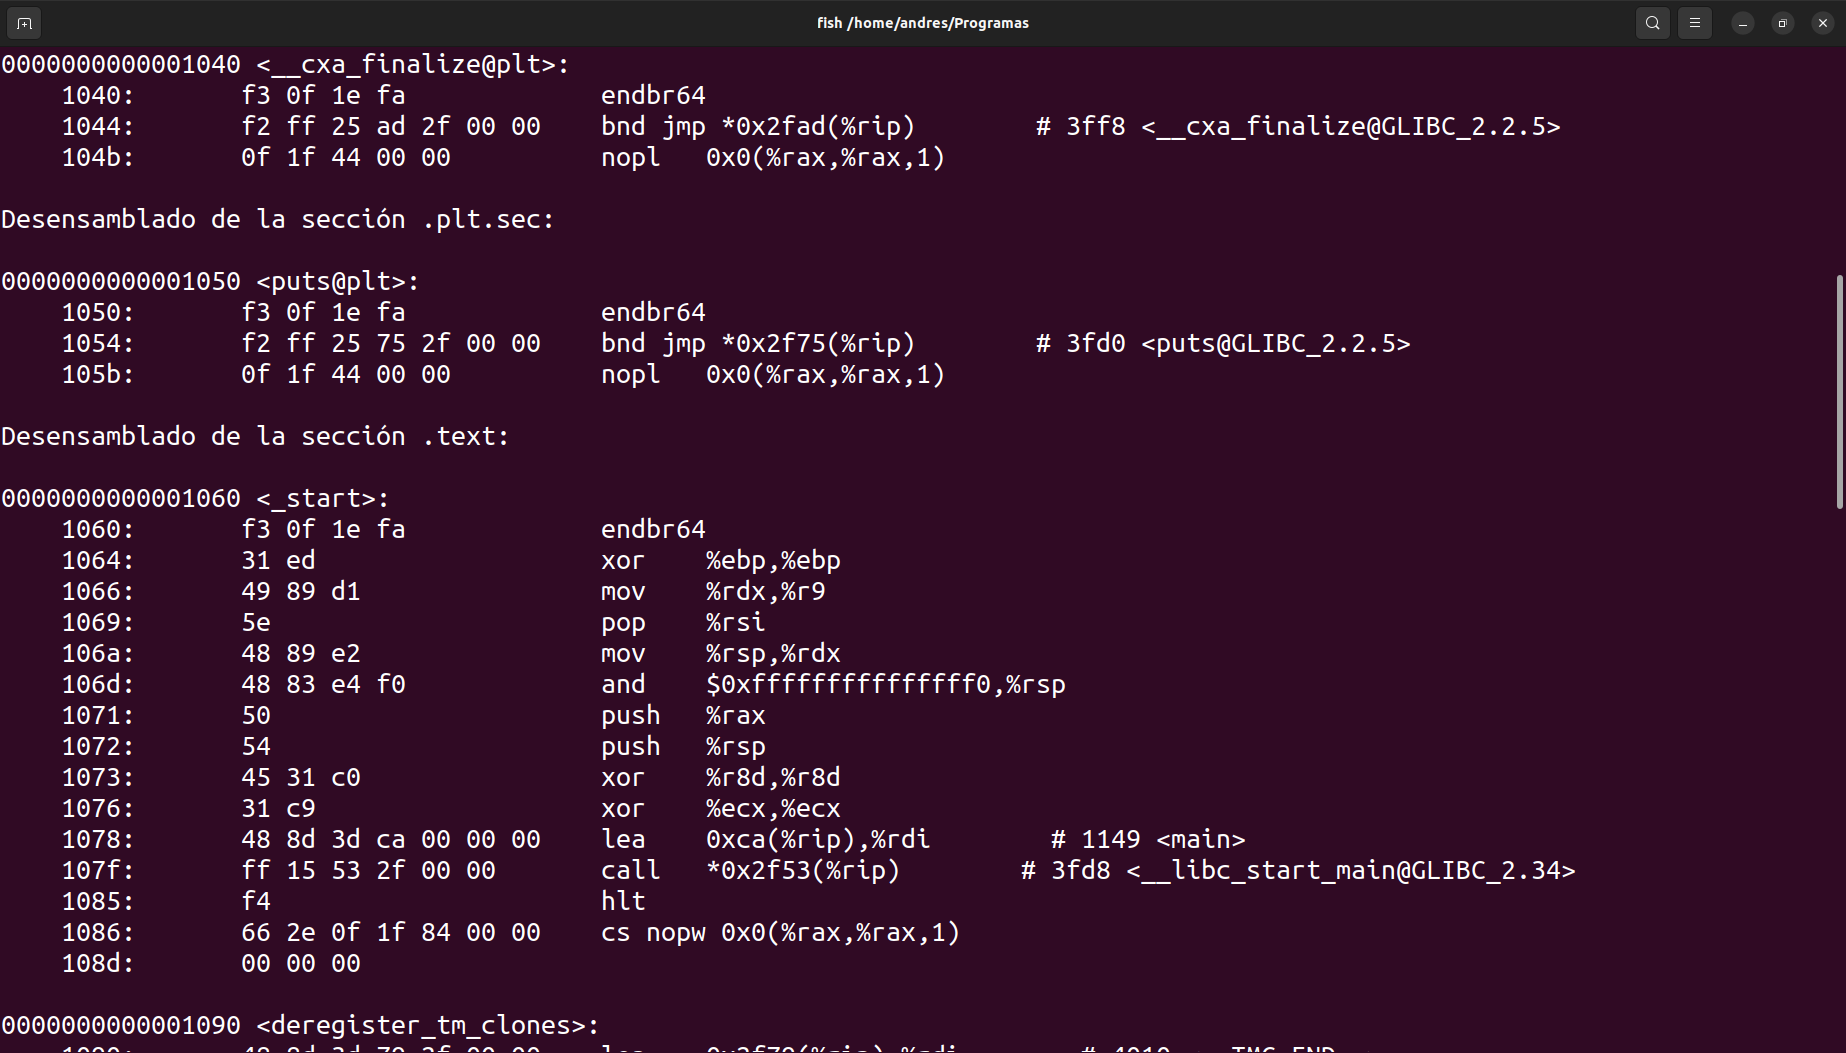
\includegraphics[width=\textwidth]{imagenes/Captura desde 2022-11-17 17-53-55.png}
    \caption{Salida producida por el comando \texttt{objdump -d salidaC}, se puede ver la llamada a \texttt{main} en \texttt{$<$\_start$>$}}
\end{figure}


\begin{figure}[H]
    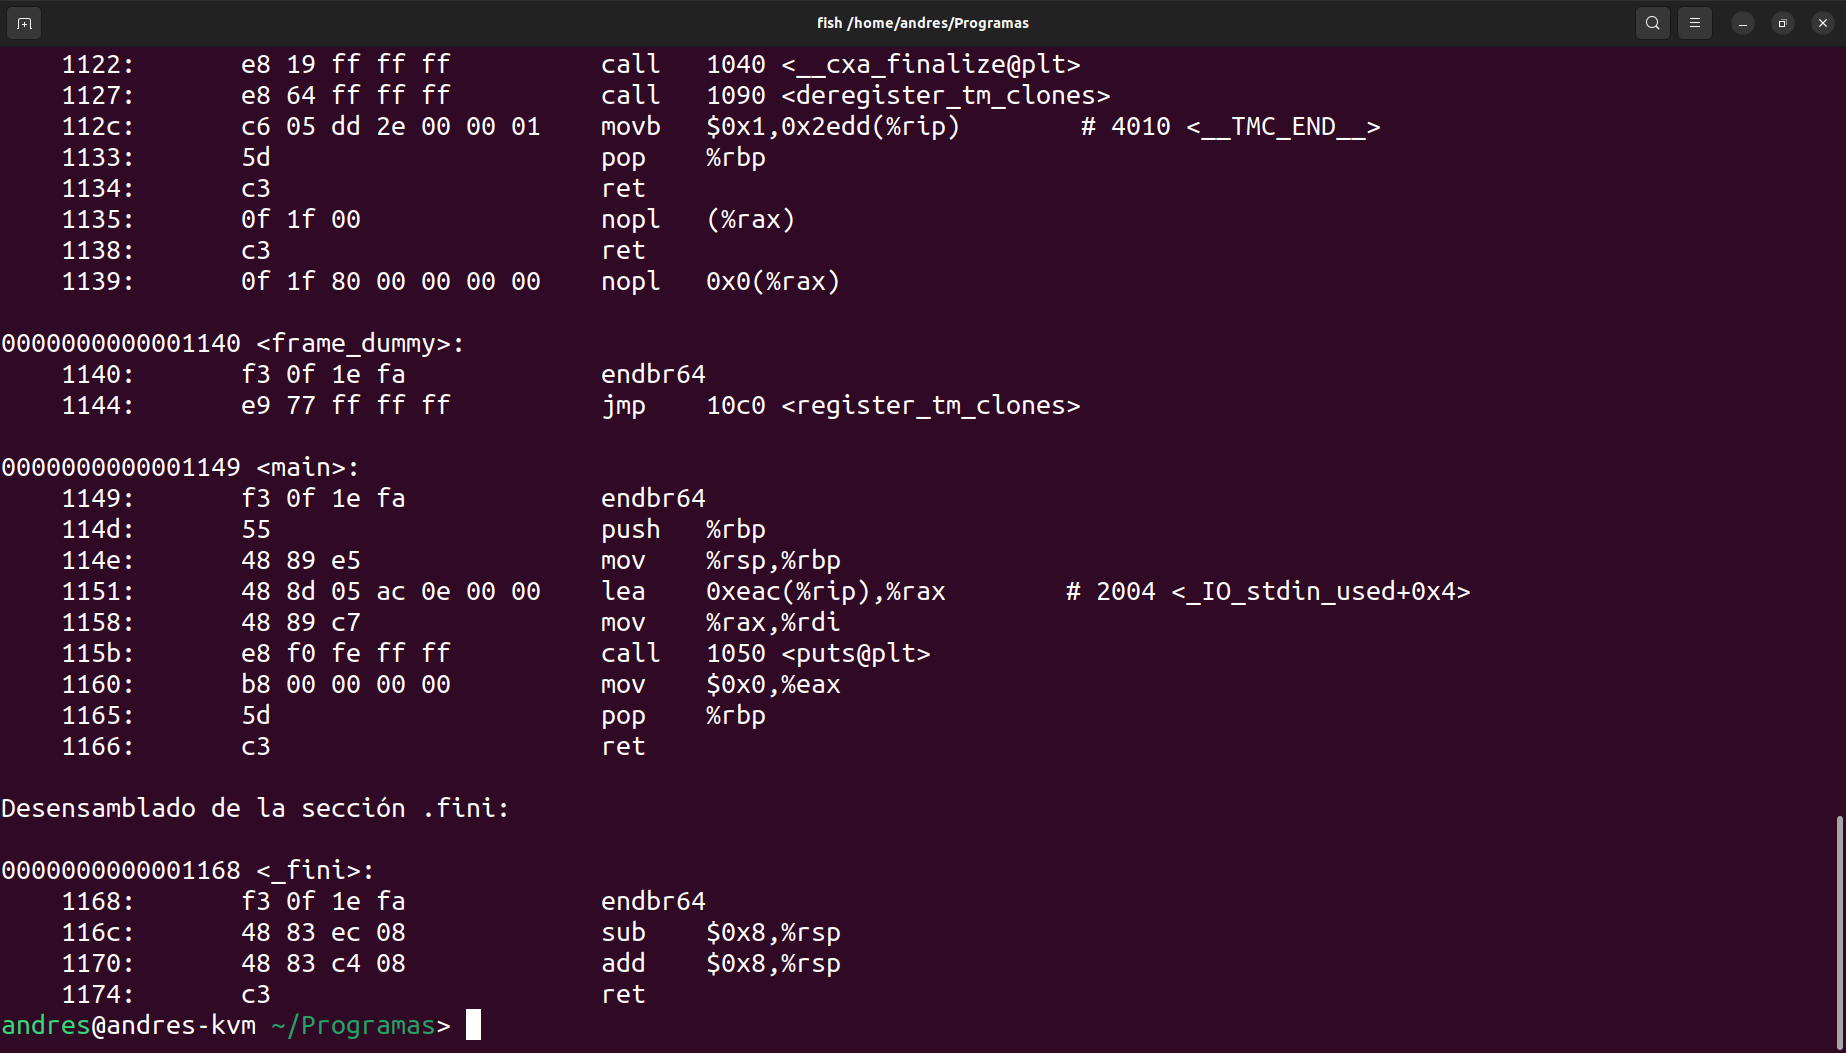
\includegraphics[width=\textwidth]{imagenes/Captura desde 2022-11-17 17-56-56.png}
    \caption{Función \texttt{$<$main$>$} compilada a de C a ensamblador.}
\end{figure}

Esto simplifica mucho el trabajo, ya que no es necesario buscar en los manuales de los procesadores que instrucción tiene cada código. Además, esto permite buscar vulnerabilidades en el programa o incluso el estudio de las distintas condiciones para que continúe el código para luego poder intentar saltarse las medidas de seguridad.

\bigskip

\section{Ejercicio 3}

\textbf{Enunciado: }``Modifica el programa realizado en el ejercicio anterior para que el programa se detenga durante un rato, por ejemplo, con un \texttt{sleep()}, al objeto de que podamos visualizar el archivo \textit{/proc/$<$PID$>$/maps} de su ejecución. Ahora analiza la información de su ELF para entrever cómo se ha construido dicho proceso a través de la información del ELF, por ejemplo, las direcciones y permisos de las regiones de texto y datos, etc.''

\bigskip

He realizado la siguiente modificación al programa en su versión C:

%modificacion del rpograma con sleep
\begin{figure}[H]
    \centering
    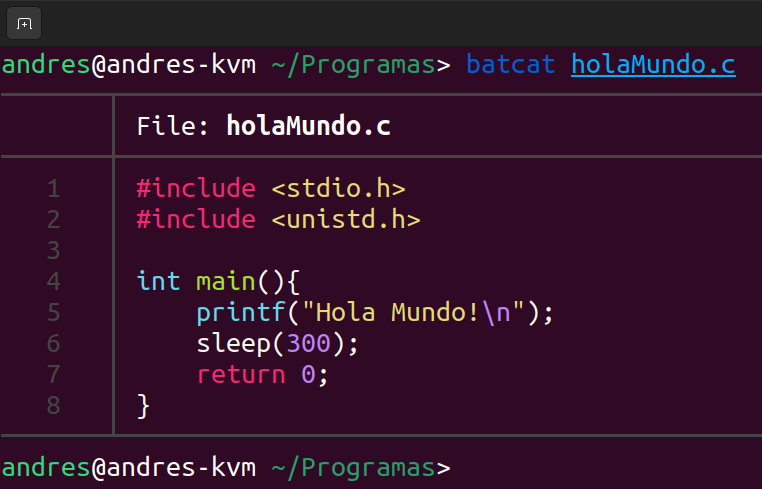
\includegraphics[width=0.7\textwidth]{imagenes/Captura desde 2022-11-17 18-12-25.png}
    \caption{Modificación realizada al programa.}
\end{figure}

\newpage

Ahora, mediante el símbolo ``\&'' se puede ejecutar el programa en segundo plano. A continuación, se busca el proceso pasando la salida de la orden \verb|ps -e| mediante un pipe a la orden \verb|grep|. Por tanto, en mi caso, la orden para encontrar el PID del programa sería así: \texttt{ps -e $\vert$ grep hola}.

%salida de ps
\begin{figure}[H]
    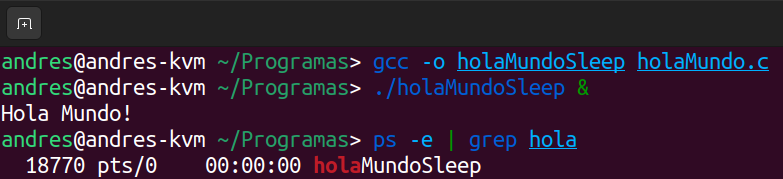
\includegraphics[width=\textwidth]{imagenes/ps.png}
    \caption{Detección del PID usando la orden \texttt{ps}.}
\end{figure}


Y sabiendo que tiene el PID \textbf{18770}, con cualquier orden para mostrar texto como \texttt{nano, cat, bat} se puede ver lo que contiene.

%salida de proc pid maps
\begin{figure}[H]
    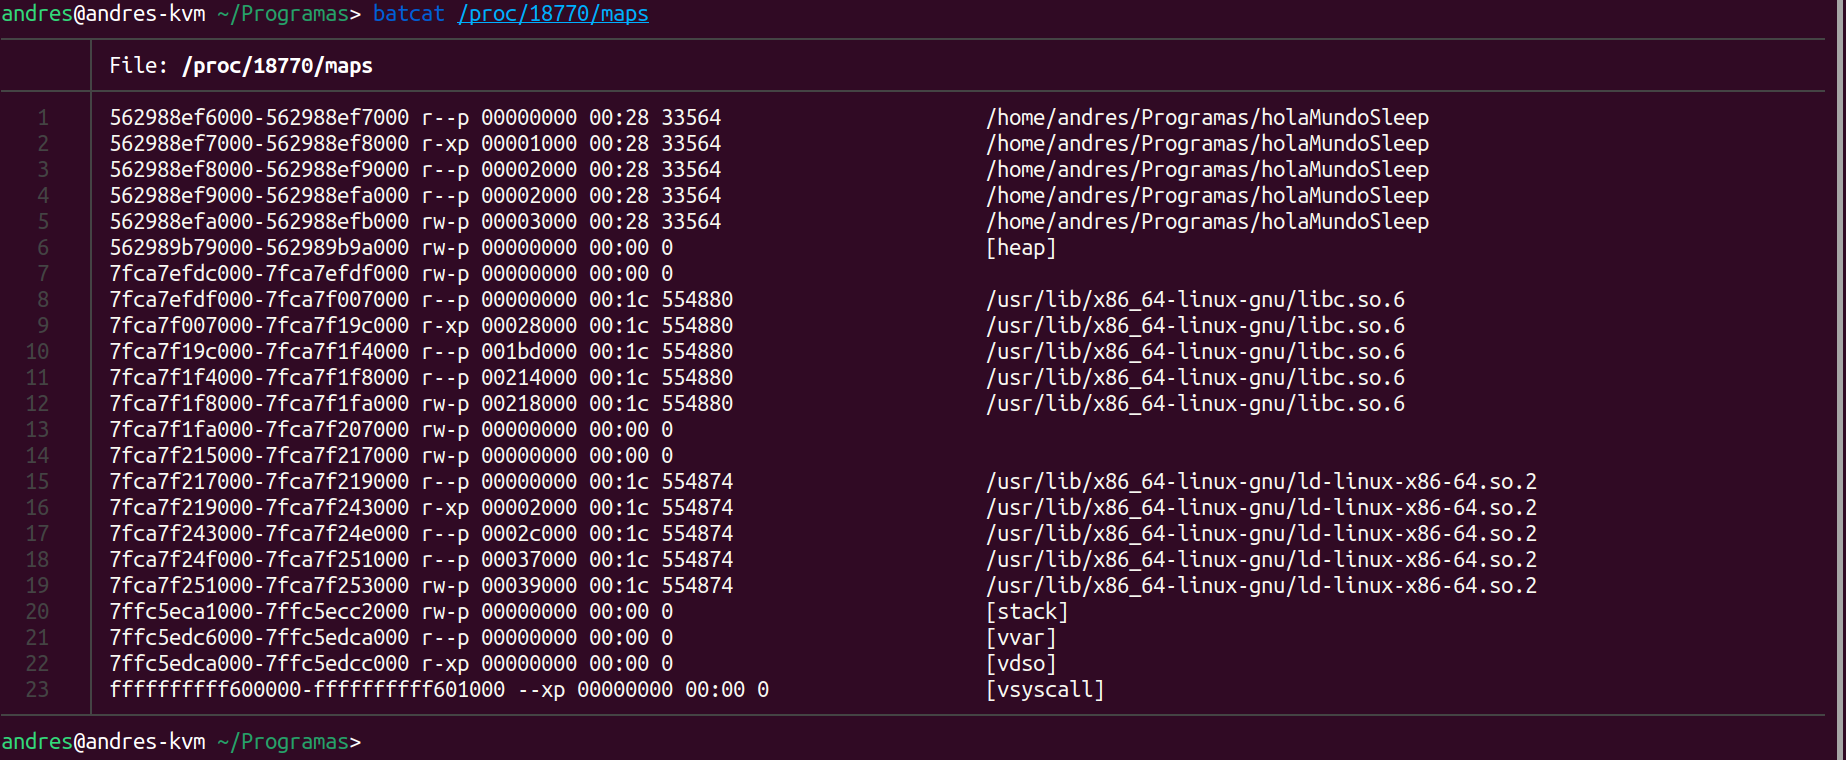
\includegraphics[width=\textwidth]{imagenes/procPID.png}
    \caption{Contenido del archivo del directorio \texttt{/proc/PID/maps}.}
\end{figure}

\newpage

Ahora, con la orden \verb|readelf -S <archivo>| podemos ver las secciones que componen el ejecutable:

%foto de la salida
\begin{figure}[H]
    \centering
    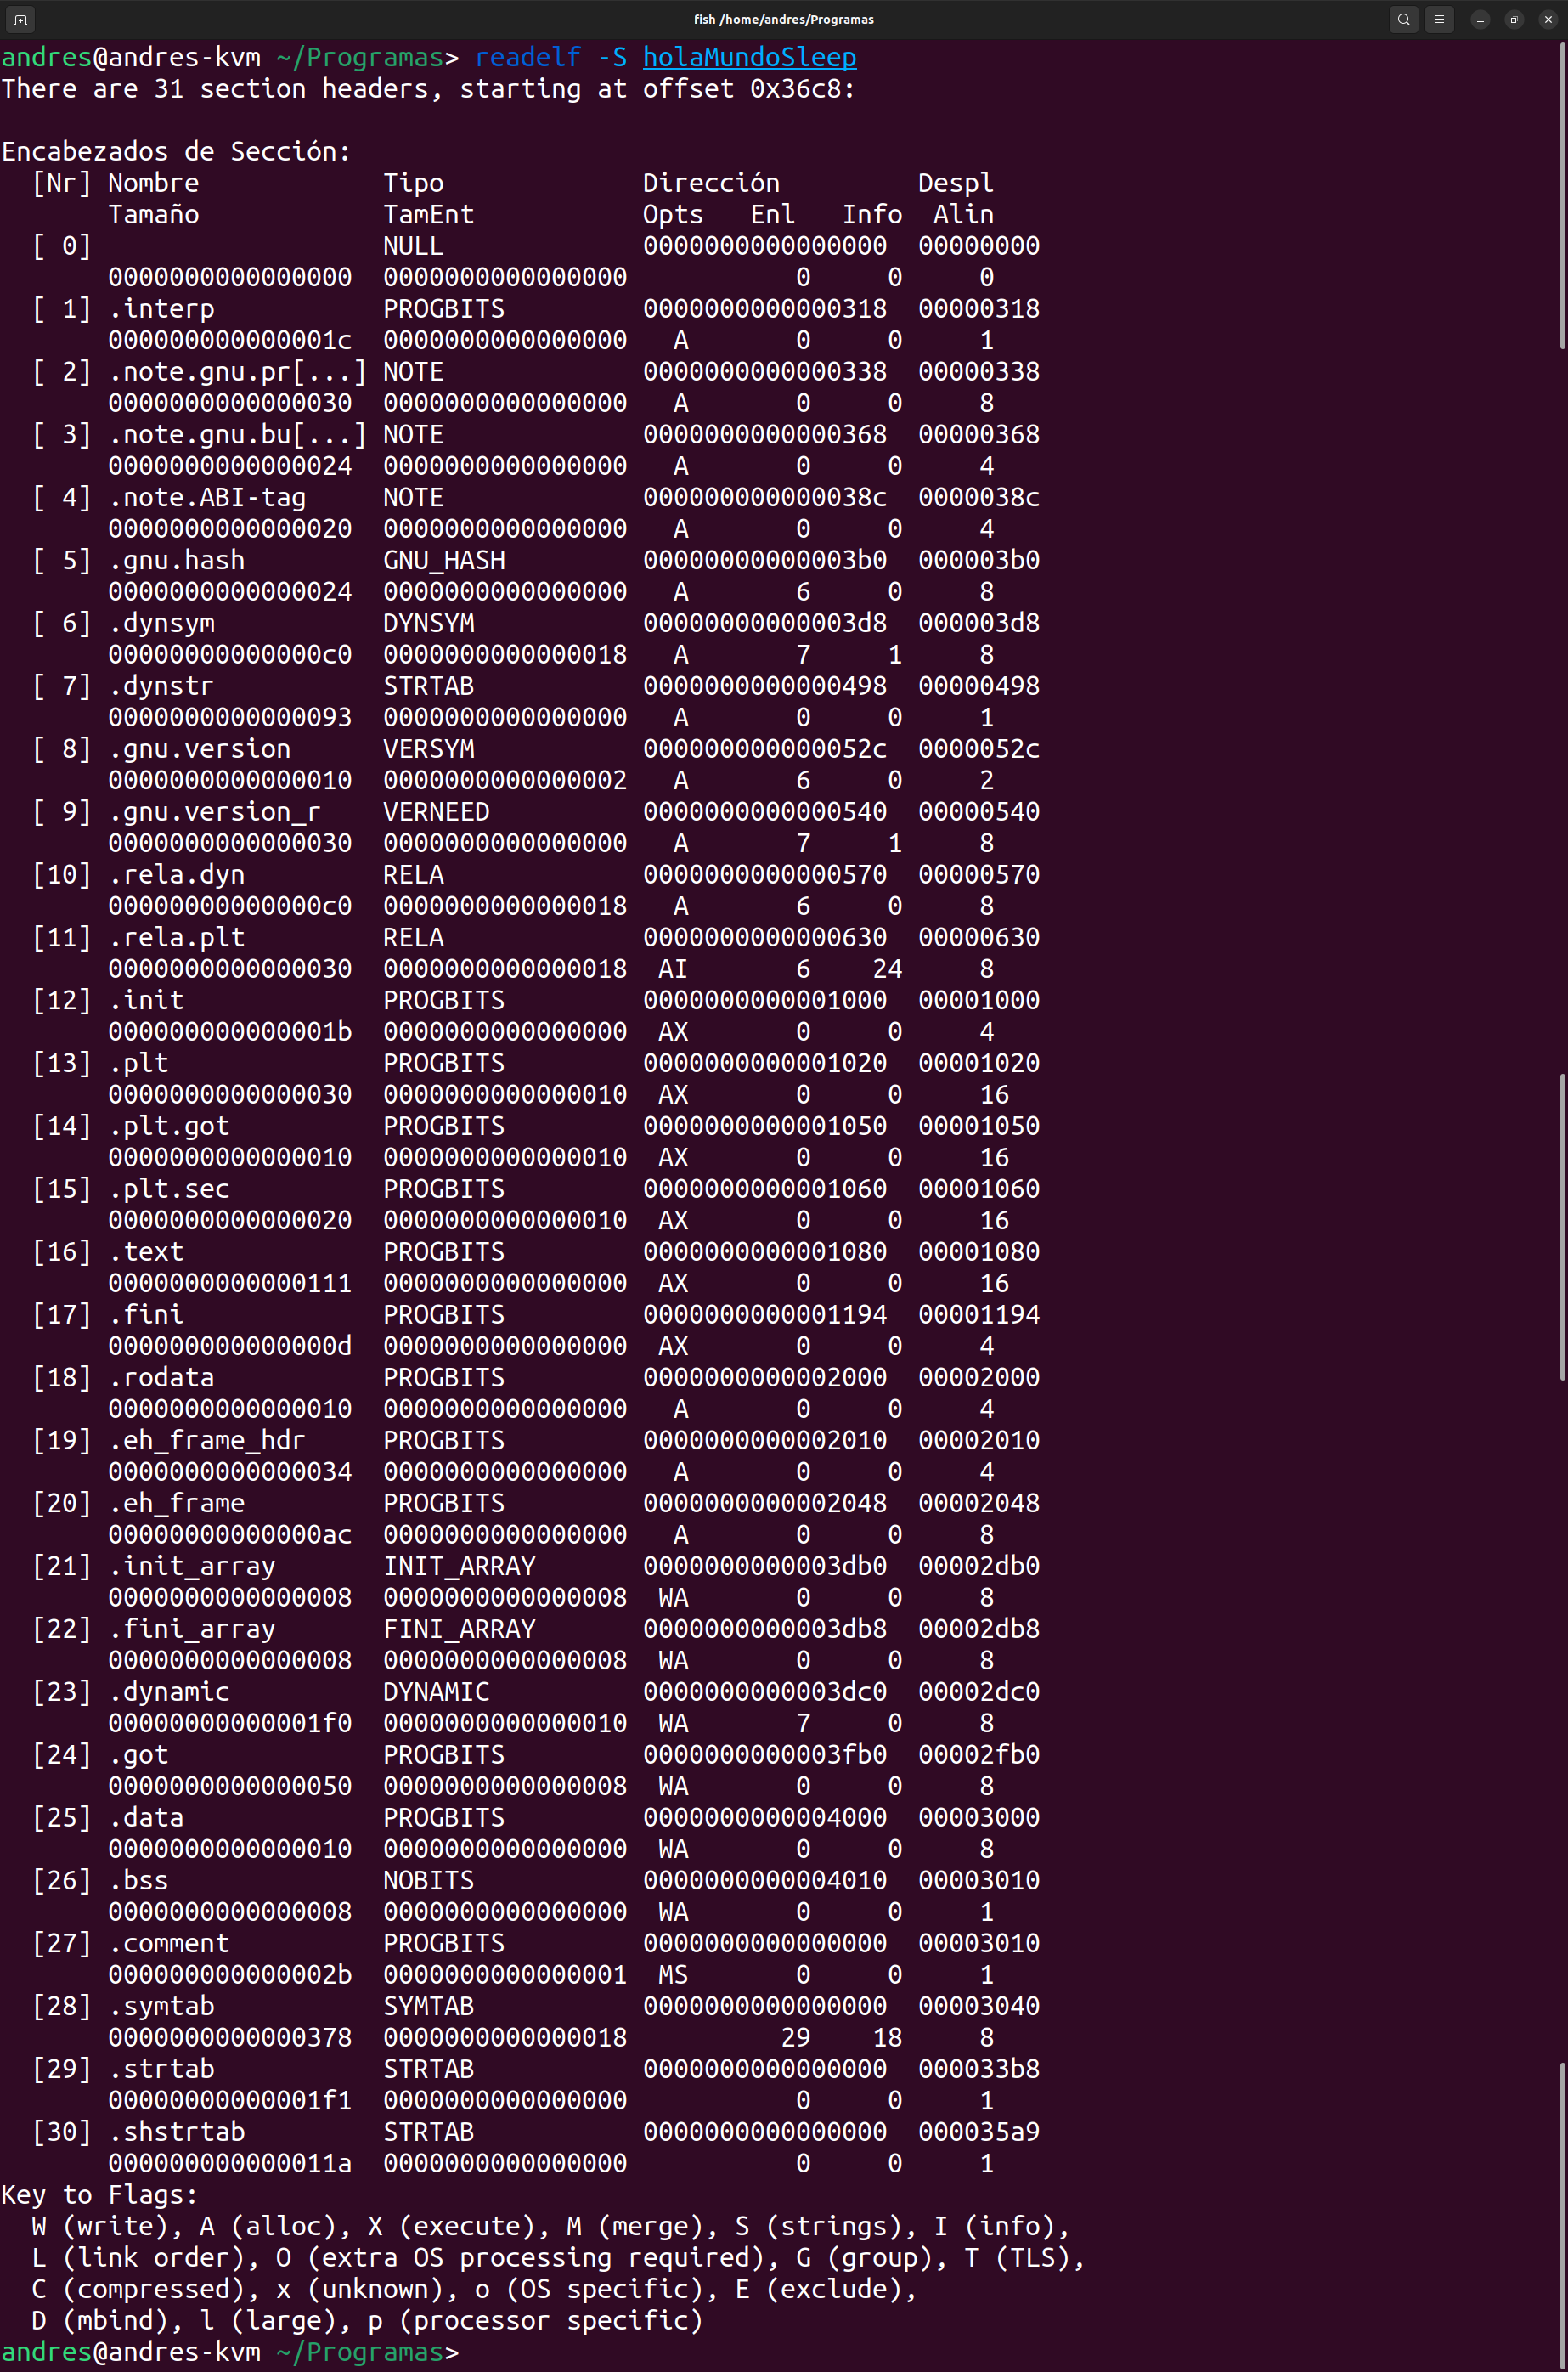
\includegraphics[width=0.8\textwidth]{imagenes/readelfSsleep.png}
    \caption{Secciones que componen el ejecutable.}
\end{figure}

\newpage

Usando la orden \verb|readelf -Wl <archivo>| se pueden obtener las cabeceras del programa.

%foto
\begin{figure}[H]
    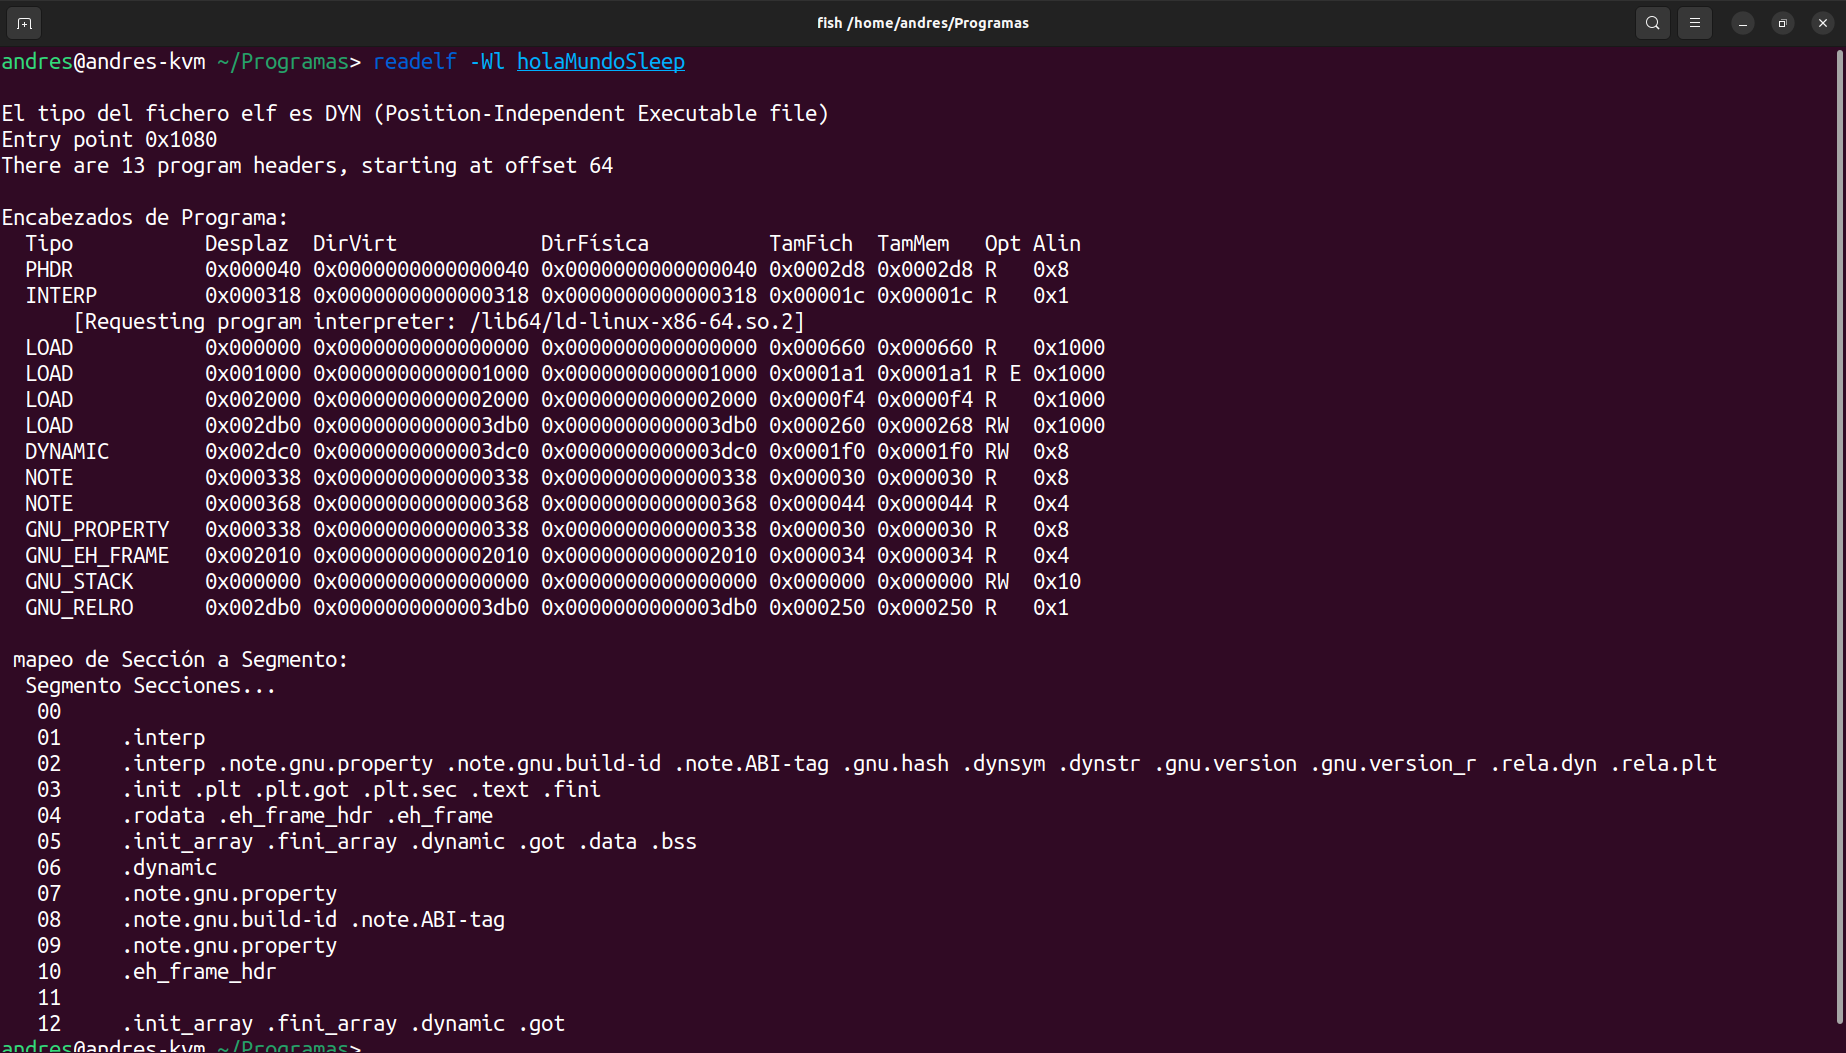
\includegraphics[width=\textwidth]{imagenes/Captura desde 2022-11-17 18-38-45.png}
    \caption{Cabeceras del programa.}
\end{figure}

\newpage

Como en el ejercicio anterior, la salida es la misma usando el comando \verb|objdump -p|:

%salida de objdump
\begin{figure}[H]
    \centering
    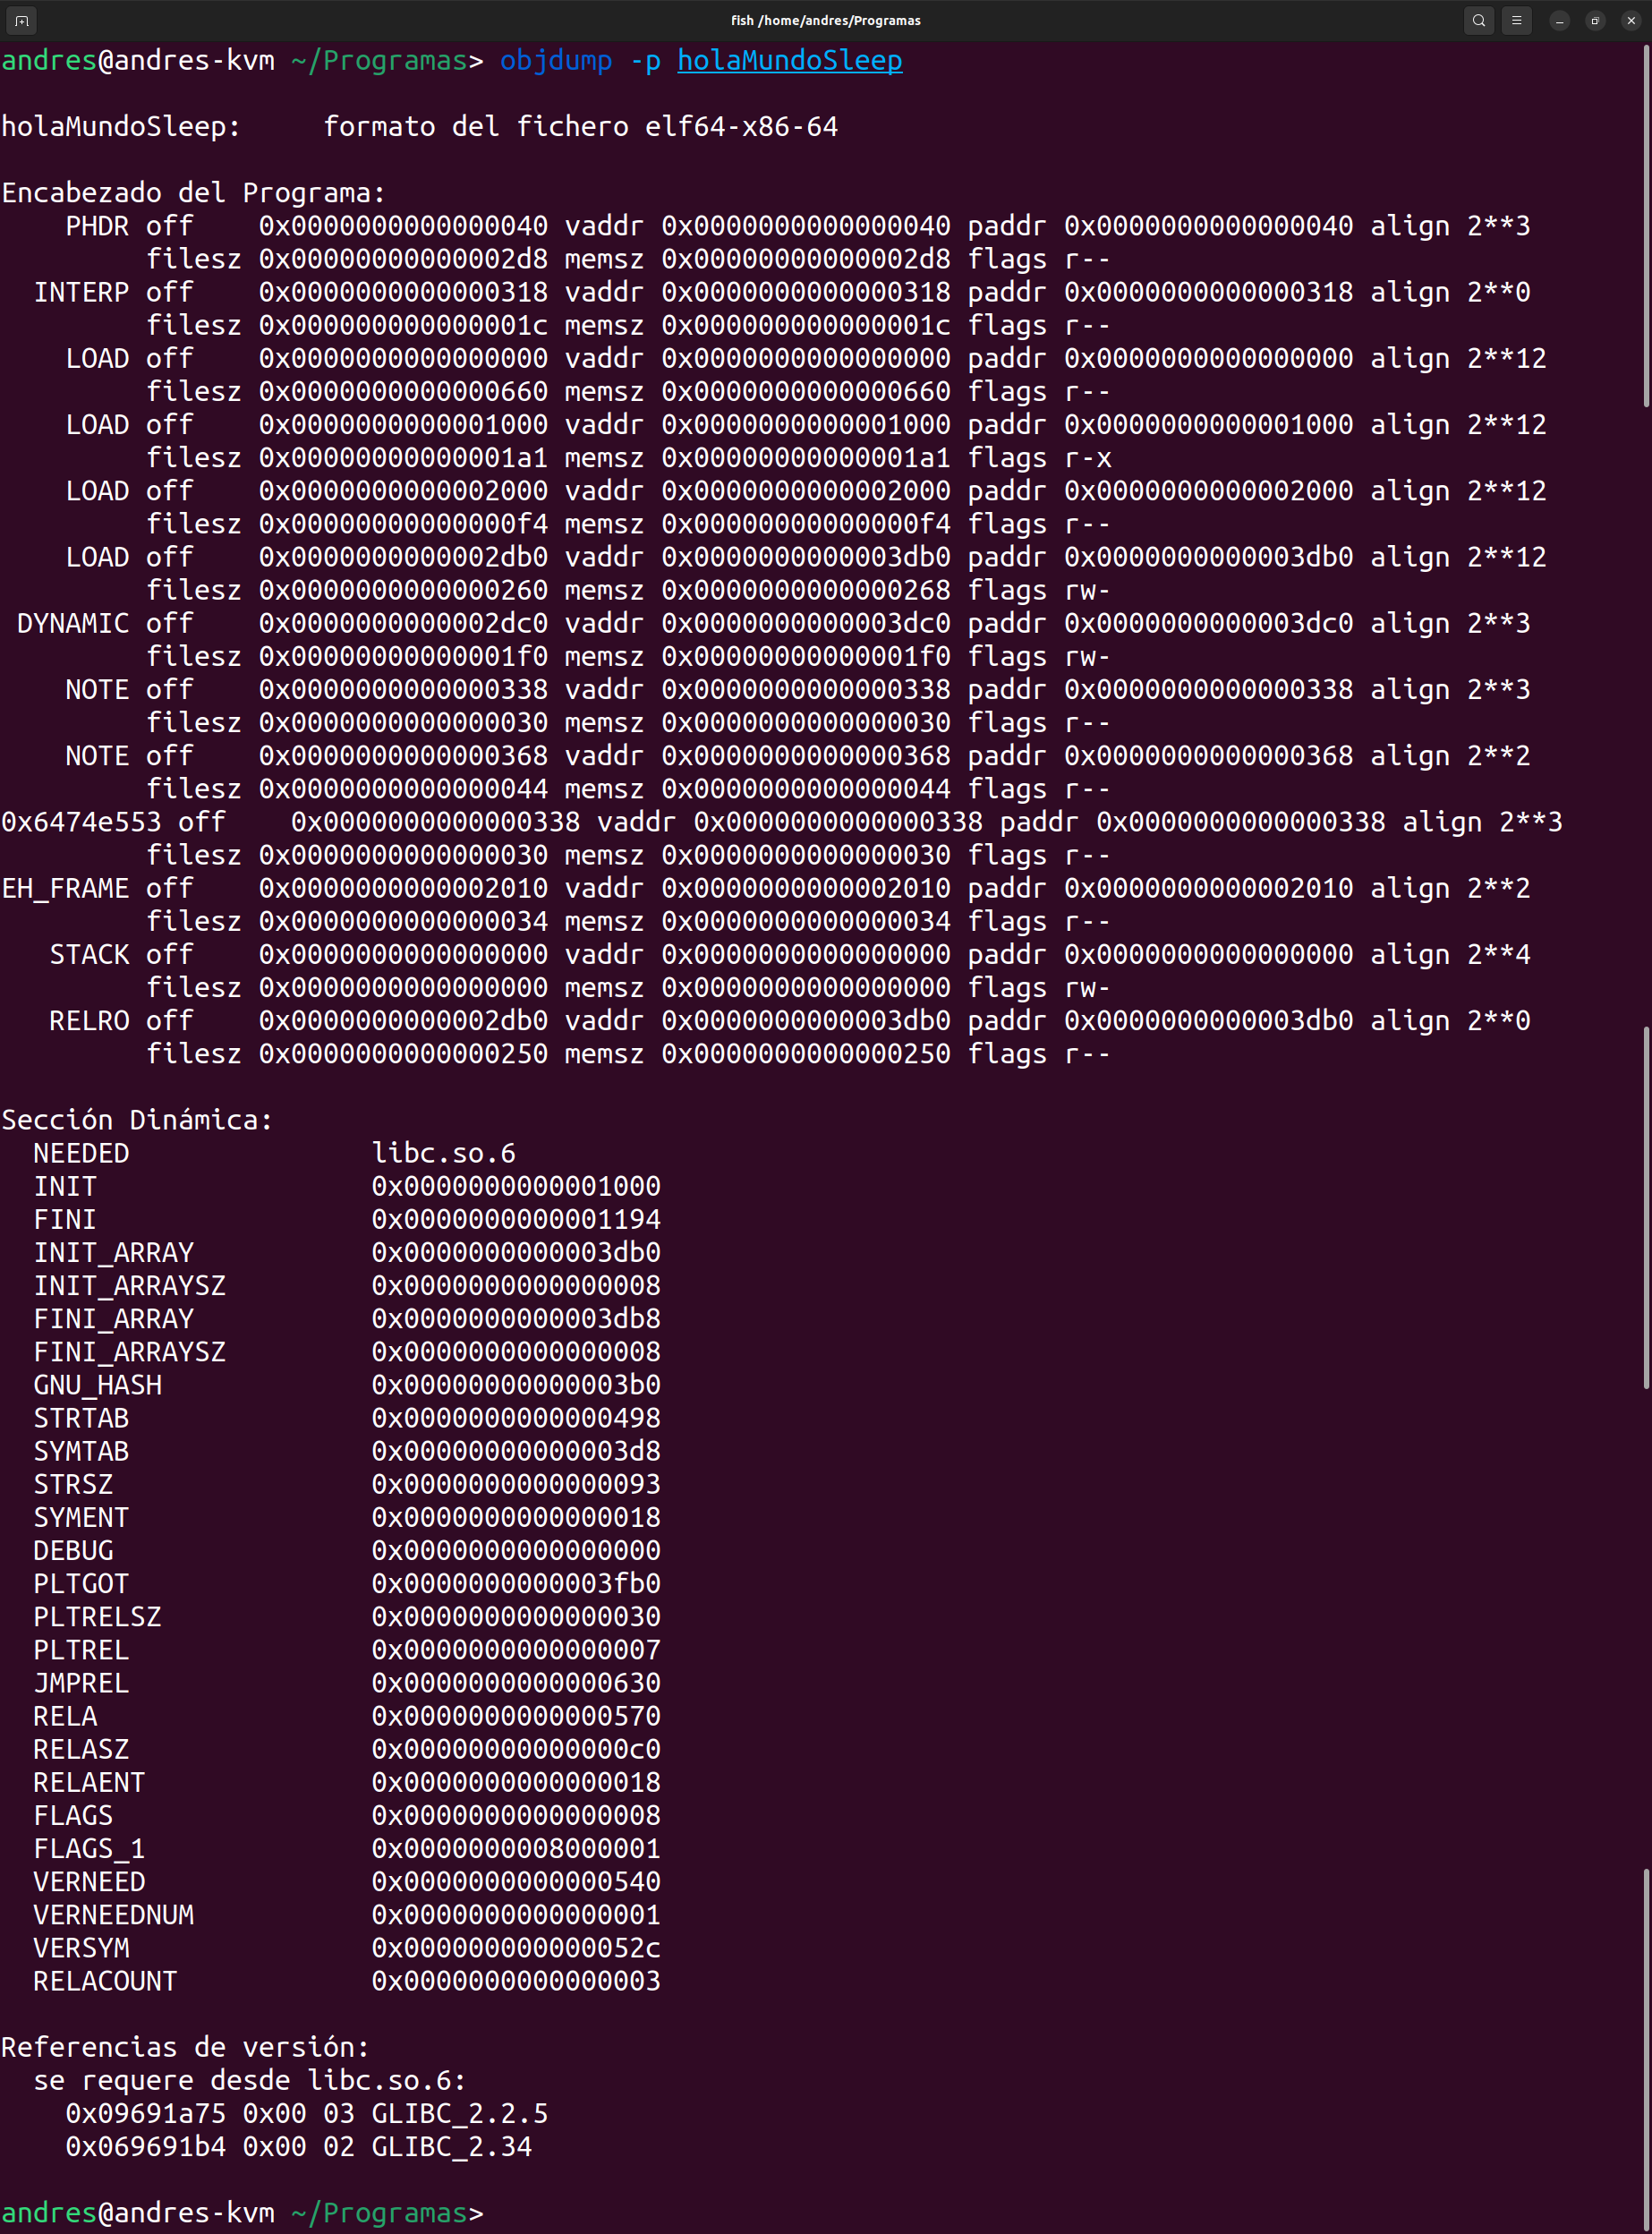
\includegraphics[width=0.7\textwidth]{imagenes/objdumppsleep.png}
    \caption{Salida del comando.}
\end{figure}

El kernel cuando ve \texttt{INTERP}, carga el primer \texttt{LOAD}, después los segmentos del programa interprete y finalmente se cargan las bibliotecas especificadas en \texttt{LD\_PRELOAD} y los segmentos \texttt{DYNAMIC}. 

\newpage

Estos segmentos dinámicos que se cargan se pueden ver con la orden \verb|readelf -d <archivo>|.

%foto de la salida
\begin{figure}[H]
    \centering
    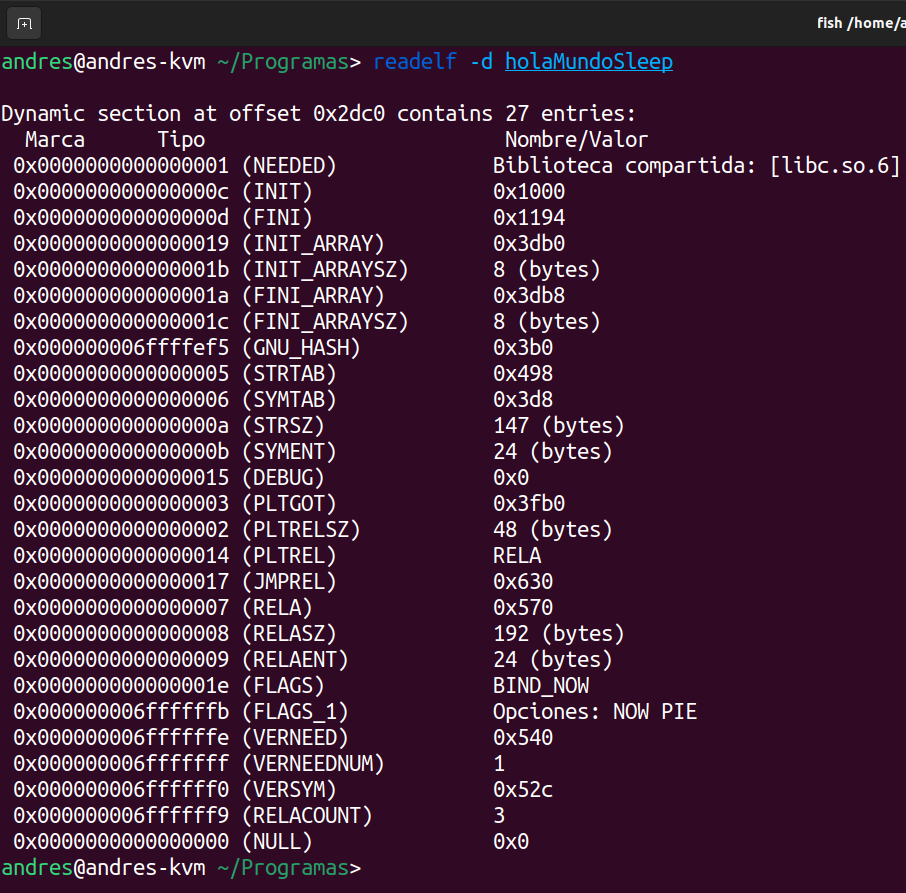
\includegraphics[width=0.7\textwidth]{imagenes/Captura desde 2022-11-17 18-47-41.png}
    \caption{Segmentos dinámicos usados por el programa.}
\end{figure}


\end{document}
